\documentclass[twoside, a4paper, 10pt]{report}
\usepackage[italian]{babel}
\usepackage[utf8]{inputenc}
\usepackage[T1]{fontenc}
\usepackage[margin=1in]{geometry}
\usepackage{graphicx}
\usepackage{fancyhdr}
\usepackage{array}
\usepackage{colortbl}
\usepackage{lastpage}
\usepackage{titlesec}
\usepackage{float}
\usepackage{subcaption}
\usepackage{hyperref}
\usepackage{afterpage}
\usepackage{minted}
\usepackage{dirtree}
\usepackage{tabularx}
\usepackage{ltablex}
\usepackage{xltabular}

% Ridefinizione per il titolo dei capitoli
\titleformat{\chapter}[hang]{\LARGE\bfseries}{\thechapter}{1em}{} 
\titlespacing{\chapter}{0pt}{0pt}{1em}

% Definizione della path per le immagini
\graphicspath{{../images/}}

% Set the version of the document
\newcommand{\version}{0.1}
\newcommand{\ProjectTitle}{SatisTrento}
\newcommand{\ProjectTitleShort}{satisTrento}
\newcommand{\FileName}{D3-\ProjectTitleShort-sviluppo}

% Definizione dei dati del documento
\title{Documento di sviluppo - \ProjectTitle}
\author{Facchini Luca, Prigione Luca, Faa Enrico}
\date{A.A. 2024/2025}

% Definizione metadati PDF
\hypersetup{
    pdftitle={\ProjectTitle},
    pdfauthor={Facchini Luca, Prigione Luca, Faa Enrico},
    pdfsubject={Sviluppo dell'applicazione \ProjectTitle},
    pdfkeywords={\ProjectTitle, Sviluppo, Comune di Trento, UniTN}
}

% Definizione counter Requisiti Funzionali
\newcounter{rfCounter}
\newcounter{rnfCounter}

% Definisci un nuovo comando per il formato RF/RNF
\newcommand{\RF}{RF\arabic{rfCounter}}
\newcommand{\RNF}{RNF\arabic{rnfCounter}}

% Definizione nuovo comando per lista con RF/RNF automatici in modo che NON si resettino ad ogni lista
% Ambiente per la lista di RF
\newenvironment{rfList}{
    \begin{list}{\textbf{\RF:}}{ \setlength{\itemsep}{0pt} } % Lista RF
        \setcounter{rfCounter}{\value{rfCounter}} % Mantieni il valore corrente
}{\end{list}}

% Ambiente per la lista di RNF
\newenvironment{rnfList}{
    \begin{list}{\textbf{\RNF:}}{ \setlength{\itemsep}{0pt} } % Lista RNF
        \setcounter{rnfCounter}{\value{rnfCounter}} % Mantieni il valore corrente
}{\end{list}}

% comandi per gli item delle liste RF e RNF
\newcommand{\rfItem}{\stepcounter{rfCounter}\item}
\newcommand{\rnfItem}{\stepcounter{rnfCounter}\item}

% Rimozione scritta "Capitolo" dai titoli dei capitoli
\renewcommand{\chaptermark}[1]{%
    \markboth{
        \thechapter.\ #1%
    }{}%
}
% Definizione del layout della pagina
\fancypagestyle{stdPage}{
    \setlength{\headheight}{24.0pt} 
    \renewcommand{\footrulewidth}{0.4pt}
    \fancyhead{}
    \fancyfoot{}
    \fancyhead[LO,RE]{\begin{tabular}{l l}
        \textbf{Document:} & Sviluppo \\
        \textbf{Version:} & \version
    \end{tabular}}
    \fancyfoot[LO,RE]{\thepage / \pageref*{LastPage}}
    \fancyhead[LE,RO]{\leftmark}
}
\fancypagestyle{eccScopo}{
    \pagestyle{stdPage}
    \fancyhead[LE,RO]{Scopo del documento}
}

\fancypagestyle{plain}{
    \pagestyle{stdPage}
}
\fancypagestyle{index}{
    \pagestyle{stdPage}
    \fancyfoot[LO,RE]{\thepage}
}

\fancypagestyle{emptyPage}{
    \setlength{\headheight}{24.0pt} 
    \renewcommand{\headrulewidth}{0pt}
    \fancyhead{}
    \fancyfoot{}
}

% Definizione della pagina bianca
\newcommand\blankpage{%
    \null
    \thispagestyle{empty}%
    \addtocounter{page}{-1}%
    \newpage
}

\begin{document}
    \pagestyle{fancy}
    \pagenumbering{Roman} 
    
    \begin{titlepage}
        \thispagestyle{emptyPage}
        
\includegraphics[width=0.33\textwidth]{logoUni.png}
        \vspace{1cm}\newline
        \textbf{Progetto:}
        \vspace{0.5cm}
        \begin{center}
            \textbf{\Huge{\ProjectTitle}}
        \end{center}
        \vspace{1cm}
        \textbf{Titolo del documento:}
        \vspace{0.5cm}
        \begin{center}
            \textbf{\huge{Sviluppo}}
        \end{center}
        \vspace{1cm}
        \textbf{Document Info}
        \vspace{0.5cm}
        % Table with document info
        \begin{center}
            \begin{tabular}{|l|l|l|c|}  
                \hline
                {\cellcolor[rgb]{0,0.502,1}}\textcolor{white}{\textbf{Doc. Name}}   & \FileName & {\cellcolor[rgb]{0,0.502,1}}\begin{tabular}[c]{@{}>{\cellcolor[rgb]{0,0.502,1}}l@{}}\textcolor{white}{\textbf{Doc.}}\\\textcolor{white}{\textbf{Number}}\end{tabular} & D3 V\version  \\ 
                \hline
                {\cellcolor[rgb]{0,0.502,1}}\textcolor{white}{\textbf{Description}} & \multicolumn{3}{l|}{Documento di sviluppo dell'applicazione} \\
                \hline
            \end{tabular}
        \end{center}
        % Document authors (1 per line) with name and ID aligned to the right but with some space from the right border 
        \vspace{1.5in}
        \vfill
        \begin{flushright}
            \rightskip=2cm
            \begin{tabular}{r l}
                \multicolumn{2}{c}{\textbf{Authors}} \\
                Facchini Luca & 245965 \\
                Prigione Luca & 242880 \\
                Faa Enrico & 243889
            \end{tabular}
        \end{flushright}
        \vfill
    \end{titlepage}
    \afterpage{\blankpage}
    \begingroup
        \setcounter{tocdepth}{1}
        \tableofcontents
        \thispagestyle{index}
    \endgroup
    \afterpage{\blankpage}
    \pagestyle{stdPage}
    
    \newpage
    \pagenumbering{arabic} 

    \chapter*{Scopo del documento}
\addcontentsline{toc}{chapter}{Scopo del documento}
\fancyhead[RE,LO]{\scshape Scopo del documento}
    \chapter{User Stories}
    \chapter{\textit{User Workflow}}
Nella seguente parte del documento verrà illustrato lo ``\textit{user flow}'' per gli utenti del tipo: ``non loggato'', ``analista'' e ``sondaggista''.
\paragraph{Utenti ``non loggati''} Come possiamo osservare dalla figura \ref{fig:UserWorkflow}, gli utenti non loggati possono visualizzare la \textit{HomePage} della applicazione web, da questa possono visualizzare i dati generici della città. In alternativa alla pressione di una zona all'interno della mappa il sistema restituirà la pagina di dettaglio della zona selezionata dalla quale possono o tornare alla \textit{HomePage} o visualizzare i dettagli. Dalla \textit{HomePage} è possibile inoltre premere sul pulsante per il passaggio da ``quartieri'' a ``circoscrizioni'' e viceversa. La mappa presente nella \textit{HomePage} è interattiva e permette di spostare la visuale e di ingrandire o rimpicciolire la mappa.
\paragraph{Utenti ``loggati''} Gli utenti loggati tramite un pulsante dedicato nella \textit{HomePage} possono accedere alla pagina di \textit{login} e, inserendo le proprie credenziali, se queste sono corrette allora in base al tipo di utente questo verrà reindirizzato alla propria pagina associata. Nel caso dell'utente ``analista'' verrà reindirizzato alla HomePage con le funzionalità di analisi, mentre l'utente ``sondaggista'' verrà reindirizzato alla pagina di gestione dei sondaggi. In entrambi i casi l'utente potrà effettuare il \textit{logout} tramite un apposito menù a tendina sul quale è presente il proprio nome.
\paragraph{Utenti ``analisti''} Gli utenti di tipo ``analista'' possono visualizzare la \textit{HomePage} con le funzionalità di analisi, in particolare possono visualizzare i dati generici della città e, in alternativa alla pressione di una zona all'interno della mappa, il sistema restituirà la pagina di dettaglio della zona selezionata dalla quale possono o tornare alla \textit{HomePage} o visualizzare i dettagli. Oltre alla possibilità di cambio di visualizzazione da ``quartieri'' a ``circoscrizioni'' e viceversa, l'analista può visualizzare i dati in modalità ``tabella'' premendo sul pulsante ``mappa''/``tabella''. A differenza di tutti gli altri utenti alla pressione di una zona all'interno della mappa verrà visualizzata la pagina di dettaglio della zona selezionata per gli analisti, da questa possiamo o tornare alla \textit{HomePage} o selezionando la categoria degli attributi visualizzare i dati della zona selezionata.
\paragraph{Utenti ``sondaggista''}
Gli utenti di tipo ``sondaggista'' dalla pagina di gestione dei sondaggi possono visualizzare lo storico dei sondaggi oppure crearne uno inserendo il titolo di questo e premendo sul pulsante ``Crea un nuovo sondaggio'', è anche possibile caricare un sondaggio precedentemente creato selezionando il file e premendo sul pulsante ``Carica sondaggio''. Dalla pagina di gestione dei sondaggi è visualizzata una tabella con i sondaggi creati dall'utente, per ogni sondaggio non ancora ``completato'' è possibile continuare la compilazione premendo sopra questo, si apre dunque la pagina di gestione del sondaggio. Da questa pagina è possibile da una serie di pulsanti terminare il sondaggio e caricarlo per l'approvazione degli amministratori (col pulsante ``Termina e Carica il Sondaggio''), premere sul pulsante ``Salva ed Esci'' per salvare i cambiamenti fatti al sondaggio e tornare alla pagina dei sondaggi, oppure premere sul pulsante ``Elimina Sondaggio'' e dopo una conferma il sondaggio verrà eliminato, anche in questo caso si verrà reindirizzati alla pagina dei sondaggi. Oltre a queste azioni è possibile eseguire le azioni di voto, questo compilando i dati del cittadino che sta per votare e premendo sul pulsante ``Vota'', al termine delle operazioni si verrà reindirizzati alla pagina di gestione del sondaggio. Se sono stati commessi errori durante la compilazione del sondaggio è possibile cancellare un voto individuale.
\begin{figure}
    \centering
    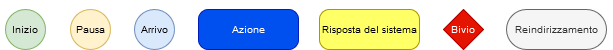
\includegraphics[width=0.9\textwidth]{User_workflow/legendeUF.png}
    \caption{User Workflow Legend}
    \label{fig:UserWorkflowLegend}
\end{figure}
\begin{figure}
    \centering
    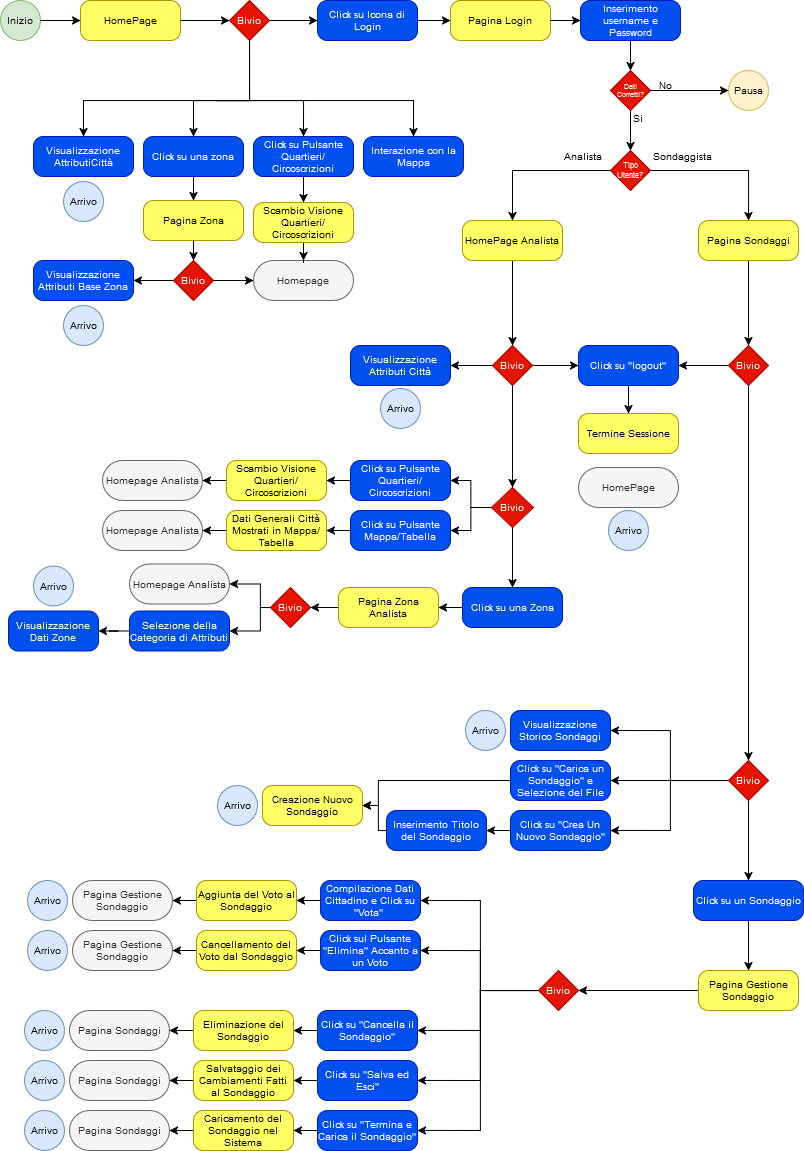
\includegraphics[width=\textwidth]{User_workflow/UserFlowComp.drawio.png}
    \caption{User Workflow}
    \label{fig:UserWorkflow}
\end{figure}
    \chapter{\textit{Web \texttt{APIs}}}
Le specifiche delle \texttt{APIs} sono state definite secondo le specifiche \texttt{OpenAPI 3.0.3} e disponibili pubblicamente presso \texttt{APIary} al seguente indirizzo: \url{https://satistrento.docs.apiary.io}.

\paragraph{Progettazione e note di design} In fase di progettazione si è scelto di ridurre al minimo la duplicazione degli attributi e delle relazioni tra le entità, in modo da rendere più semplice la manutenzione e l'aggiornamento delle \texttt{APIs} in futuro, dunque è presente un elevato numero di componenti ed ereditarietà tra questi. Inoltre si è seguito il paradigma degli ``\texttt{API} link'' per permettere una navigazione più semplice e intuitiva tra le risorse.

\paragraph{Specifiche} Le specifiche delle \texttt{APIs} sono disponibili al seguente indirizzo: \url{https://github.com/lucafano04/progettoComune/blob/main/APIdoc/api.yaml} e sono riportate di seguito.


\begin{minted}[
  linenos,
  breaklines,
  tabsize=2,
  fontsize=\footnotesize
]{yaml}
openapi: 3.0.3
info:
  title: Documentazione API progetto "SatisTrento"
  description: Documentazione API per il progetto "SatisTrento" all'interno del progetto "100 progetti per il comune di Trento" per il corso di Ingegneria del Software a.a. 2024/2025 corso di laurea in Informatica presso l'Università degli Studi di Trento.
  version: 0.0.1
servers:
  - url: http://localhost:3000/api/v1
    description: Development server for testing
  - url: https://progettocomune.onrender.com/api/v1
    description: Production server

components:
  schemas:
    DatiBase:
      description: Oggetto contenente le informazioni di base di un quartiere.
      type: object
      properties:
        popolazione:
            type: integer
            description: Numero di abitanti del quartiere.
        superficie:
          type: number
          description: Superficie del quartiere in km^2.
          format: double
        serviziTotali: 
          type: integer
          description: Numero totale di servizi presenti nel quartiere.
        soddisfazioneMedia:
          type: number
          description: Soddisfazione media degli abitanti del quartiere.
          format: double
          minimum: 0
          maximum: 100
        interventiPolizia: 
          type: integer
          description: Numero di interventi delle forze dell'ordine nel quartiere.
        etaMedia:
          type: number
          description: Età media degli abitanti del quartiere.
          format: double
    ServiziGenerali:
      description: Oggetto contenente le informazioni sui servizi presenti in un quartiere.
      type: object
      properties:
        areeVerdi:
          type: integer
          description: Numero di aree verdi presenti nel quartiere.
          minimum: 0
        scuole:
          type: integer
          description: Numero di scuole presenti nel quartiere.
          minimum: 0
        serviziRistorazione:
          type: integer
          description: Numero di servizi di ristorazione presenti nel quartiere.
          minimum: 0
        localiNotturni: 
          type: integer
          description: Numero di locali notturni presenti nel quartiere.
          minimum: 0
    Sicurezza:
      description: Oggetto contenente le informazioni sulla sicurezza di un quartiere.
      type: object
      properties:
        numeroInterventi:
          type: integer
          description: Numero di interventi delle forze dell'ordine nel quartiere.
          minimum: 0
        incidenti: 
          type: integer
          description: Numero di incidenti nel quartiere.
          minimum: 0
        tassoCriminalita:
          type: number
          description: Tasso di criminalità del quartiere.
          format: double
          minimum: 0
    Coordinate:
      description: Array di coordinate che definiscono un quartiere e/o circoscrizione.
      type: array
      items: 
        description: Coordinate nel formato [latitude, longitude].
        type: array
        items:
          type: number
          format: double
        minItems: 2
        maxItems: 2
      minItems: 1
      uniqueItems: true
    Soddisfazione: 
        type: "number"
        description: "Soddisfazione media degli abitanti del quartiere."
        format: "double"
        minimum: 0
        maximum: 100
    CircoscrizioneBaseNC: 
      description: Oggetto contenente le informazioni di Base di una circoscrizione. (Senza coordinate)
      type: object
      properties:
        self:
          type: string
          description: Identificatore univoco della circoscrizione.
        nome:
          type: string
          description: Nome della circoscrizione.
        soddisfazioneMedia:
          "$ref": "#/components/schemas/Soddisfazione"
    CircoscrizioneBase: 
      description: Oggetto contenente le informazioni di Base di una circoscrizione.
      type: object
      allOf:
        - "$ref": "#/components/schemas/CircoscrizioneBaseNC"
      properties:
        coordinate:
          "$ref": "#/components/schemas/Coordinate"
    Circoscrizione:
      description: Oggetto contenente le informazioni di una circoscrizione.
      allOf:
        - "$ref": "#/components/schemas/CircoscrizioneBase"
        - "$ref": "#/components/schemas/DatiBase"
      type: object
      properties:
        servizi:
          "$ref": "#/components/schemas/ServiziGenerali"
        sicurezza:
          "$ref": "#/components/schemas/Sicurezza"
    CircoscrizioneNC:
      description: Oggetto contenente le informazioni di una circoscrizione. (Senza coordinate)
      allOf:
        - "$ref": "#/components/schemas/CircoscrizioneBaseNC"
        - "$ref": "#/components/schemas/DatiBase"
      type: object
      properties:
        servizi:
          "$ref": "#/components/schemas/ServiziGenerali"
        sicurezza:
          "$ref": "#/components/schemas/Sicurezza"
    QuartiereBaseNC:
      description: Oggetto contenente le informazioni di base di un quartiere. (Senza coordinate)
      type: object
      properties:
        self:
          type: string
          description: "Url della risorsa."
        nome:
          type: "string"
          description: "Nome del quartiere."
        circoscrizione:
          "$ref": "#/components/schemas/CircoscrizioneBaseNC"
        soddisfazioneMedia:
          "$ref": "#/components/schemas/Soddisfazione"
    QuartiereBase: 
      description: Oggetto contenente le informazioni di base di un quartiere.
      type: object
      allOf:
        - "$ref": "#/components/schemas/QuartiereBaseNC"
      properties:
        circoscrizione:
          "$ref": "#/components/schemas/CircoscrizioneBase"
        coordinate:
          "$ref": "#/components/schemas/Coordinate"
    Quartiere: 
      description: Oggetto contenente le informazioni di un quartiere.
      allOf:
        - "$ref": "#/components/schemas/QuartiereBase"
        - "$ref": "#/components/schemas/DatiBase"
      type: object
      properties:
        servizi:
          "$ref": "#/components/schemas/ServiziGenerali"
        sicurezza:
          "$ref": "#/components/schemas/Sicurezza"
    QuartiereNC:
      description: Oggetto contenente le informazioni di un quartiere.
      allOf:
        - "$ref": "#/components/schemas/QuartiereBaseNC"
        - "$ref": "#/components/schemas/DatiBase"
      type: object
      properties:
        servizi:
          "$ref": "#/components/schemas/ServiziGenerali"
        sicurezza:
          "$ref": "#/components/schemas/Sicurezza"
    User:
      description: Oggetto contenente le informazioni di un utente.
      type: object
      properties:
        self:
          type: string
          description: Url della risorsa.
        email:
          type: string
          description: Email dell'utente.
        nome:
          type: string
          description: Nome dell'utente.
        cognome:
          type: string
          description: Cognome dell'utente.
        ruolo:
          type: string
          enum:
            - "amministratore"
            - "analista"
            - "sondaggista"
            - "circoscrizione"
          description: Ruolo dell'utente.
        imageUrl: 
          type: string
          description: Url dell'immagine profilo dell'utente. (gravatar)
    Session: 
      description: Oggetto contenente le informazioni di una sessione.
      type: object
      properties:
        token:
          type: string
          description: Token di autenticazione dell'utente.
        user:
          "$ref": "#/components/schemas/User"
    Error:
      description: Oggetto contenente le informazioni di un errore.
      type: object
      properties:
        code:
          type: integer
          description: Codice dell'errore.
        message:
          type: string
          description: Messaggio di errore.
        details:
          type: string
          description: Dettagli dell'errore.
          nullable: true
    AddSondaggio:
      description: Oggetto contenente le informazioni per aggiungere un sondaggio.
      type: object
      properties:
        titolo:
          type: string
          description: Titolo del sondaggio.
    SondaggioBase: 
      description: Oggetto contenente le informazioni di base di un sondaggio.
      type: object
      allOf:
        - $ref: "#/components/schemas/AddSondaggio"
      properties:
        self:
          type: string
          description: URL della risorsa.
        dataInizio:
          type: string
          description: Data di inizio del sondaggio.
          format: date
        isAperto:
          type: boolean
          description: Indica se il sondaggio è aperto (in corso) o chiuso.
        statoApprovazione:
          type: string
          enum:
            - "approvato"
            - "in attesa"
            - "rifiutato"
          description: Stato di approvazione del sondaggio.
        sondaggista:
          "$ref": "#/components/schemas/User"
    ElencoSondaggi:
      description: Array di oggetti contenenti le informazioni di base di un sondaggio (visualizzazione sondaggista/admin).
      oneOf:
        - type: array
          items:
            "$ref": "#/components/schemas/SondaggioBase"
        - type: array
          items:
            "$ref": "#/components/schemas/Sondaggio"
    AddVoto:
      description: Oggetto contenente le informazioni per aggiungere un voto.
      type: object
      properties:
        eta:
          type: integer
          description: Età dell'utente che ha effettuato il voto. Può essere null se non specificata.
          minimum: 0
          nullable: true
        voto:
          type: integer
          description: Voto assegnato al quartiere.
          minimum: 1
          maximum: 5
        quartiere:
          type: string
          description: Identificatore univoco del quartiere.
    Voto:
      description: Oggetto contenente le informazioni di un voto.
      type: object
      properties:
        self:
          type: string
          description: Identificatore univoco del voto.
        dataOra:
          type: string
          description: Data e ora in cui è stato effettuato il voto.
          format: date-time
      allOf:
        - "$ref": "#/components/schemas/AddVoto"
    MediaVoti:
      description: Oggetto semplice contenente la media dei voti di un quartiere.
      type: object
      properties:
        media:
          type: number
          description: Media dei voti assegnati al quartiere.
          format: double
          minimum: 1
          maximum: 5
        quartiere:
          type: string
          description: Identificatore univoco della risorsa del quartiere.
    Sondaggio:
      description: Oggetto contenente le informazioni di un sondaggio.
      allOf:
        - "$ref": "#/components/schemas/SondaggioBase"
      type: object
      properties:
        voti:
          type: array
          items:
            "$ref": "#/components/schemas/Voto"
          description: Array di oggetti contenenti i voti assegnati al sondaggio.
        mediaVoti:
          type: array
          items:
            "$ref": "#/components/schemas/MediaVoti"
          description: Array di oggetti contenenti la media dei voti assegnati ai quartieri presenti nel sondaggio (quelli non presenti non vengono visualizzati).
  securitySchemes:
    BearerAuth:
      type: http
      scheme: bearer
      bearerFormat: JWT
      description: Token di autenticazione fornito all'utente per accedere alle risorse specifiche protette.

paths:
  '/quartieri' :
    description: "Risorsa che restituisce la lista dei quartieri di Trento."
    get: 
      summary: "Ottieni lista dei quartieri"
      description: "Ritorna una lista di tutti i quartieri della città di Trento."
      parameters:
        - name: deepData
          in: query
          description: "Se impostato a true, restituisce le informazioni complete di ogni quartiere."
          required: false
          schema:
            type: boolean
            default: false
          allowEmptyValue: true
        - name: coordinate
          in: query
          description: "Se impostato non impostato o impostato a true restituisce le coordinate di ogni quartiere, altrimenti no."
          required: false
          schema:
            type: boolean
            default: true
          allowEmptyValue: true
      responses: 
        200: 
          description: "Risposta con la lista dei quartieri."
          content:
            application/json:
              schema: 
                oneOf:
                  - type: array
                    items: 
                      "$ref": "#/components/schemas/QuartiereBase"
                  - type: array
                    items: 
                      "$ref": "#/components/schemas/Quartiere"
                  - type: array
                    items: 
                      "$ref": "#/components/schemas/QuartiereNC"
                  - type: array
                    items: 
                      "$ref": "#/components/schemas/QuartiereBaseNC"
      tags:
        - Quartieri
        - Dati Statici
  '/quartieri/{id}' :
    description: "Risorsa che restituisce le informazioni di un quartiere di Trento con le informazioni di base e i servizi presenti."
    parameters:
      - name: id
        in: path
        description: "Identificatore univoco del quartiere."
        required: true
        schema:
          type: string
      - name: coordinate
        in: query
        description: "Se impostato a true, restituisce le coordinate del quartiere, altrimenti no. Impostato di default a true."
        required: false
        schema:
          type: boolean
          default: true
        allowEmptyValue: true
    get: 
      summary: "Ottieni informazioni di un quartiere"
      responses: 
        200:
          description: "Risposta con le informazioni del quartiere."
          content:
            application/json: 
              schema:
                oneOf:
                  - $ref: "#/components/schemas/Quartiere"
                  - $ref: "#/components/schemas/QuartiereNC"
        404: 
          description: "Quartiere non trovato."
          content: 
            application/json: 
              schema: 
                "$ref": "#/components/schemas/Error"
      tags:
        - Quartieri
        - Dati Statici
  '/circoscrizioni' : 
    description: "Risorsa che restituisce la lista delle circoscrizioni di Trento."
    get: 
      summary: "Ottieni lista delle circoscrizioni"
      description: "Returns a list of all the districts in the city of Trento."
      parameters:
        - name: deepData
          in: query
          description: "Se impostato a true, restituisce le informazioni complete di ogni circoscrizione."
          required: false
          schema:
            type: boolean
            default: false
          allowEmptyValue: true
        - name: coordinate
          in: query
          description: "Se impostato non impostato o impostato a true restituisce le coordinate di ogni circoscrizione, altrimenti no."
          required: false
          schema:
            type: boolean
            default: true
          allowEmptyValue: true
      responses:
        200 :
          description: "Successful response"
          content:
            application/json:
              schema: 
                oneOf:
                  - type: "array"
                    items: 
                      "$ref": "#/components/schemas/CircoscrizioneBase"
                  - type: "array"
                    items: 
                      "$ref": "#/components/schemas/Circoscrizione"
                  - type: "array"
                    items: 
                      "$ref": "#/components/schemas/CircoscrizioneBaseNC"
                  - type: "array"
                    items: 
                      "$ref": "#/components/schemas/CircoscrizioneNC"
      tags:
        - Circoscrizioni
        - Dati Statici
  '/circoscrizioni/{id}' :
    description: "Risorsa che restituisce le informazioni di una circoscrizione di Trento con le informazioni di base e i servizi presenti."
    parameters:
      - name: id
        in: path
        description: "Identificatore univoco della circoscrizione."
        required: true
        schema:
          type: string
      - name: coordinate
        in: query
        description: "Se impostato a true, restituisce le coordinate della circoscrizione, altrimenti no. Impostato di default a true."
        required: false
        schema:
          type: boolean
          default: true
        allowEmptyValue: true
    get: 
      summary: "Ottieni informazioni di una circoscrizione"
      responses: 
        200:
          description: "Risposta con le informazioni della circoscrizione."
          content:
            application/json: 
              schema: 
                oneOf:
                  - $ref: "#/components/schemas/Circoscrizione"
                  - $ref: "#/components/schemas/CircoscrizioneNC"
        404: 
          description: "Circoscrizione non trovata."
          content: 
            application/json: 
              schema: 
                "$ref": "#/components/schemas/Error"
      tags:
        - Circoscrizioni
        - Dati Statici
  '/generalInfo' :
    description: "Risorsa che restituisce le informazioni generali della città di Trento."
    get: 
      summary: "Ottieni informazioni generali"
      description: "Restituisce le informazioni generali della città di Trento."
      responses: 
        200 : 
          description: "Successful response"
          content: 
            application/json:
              schema: 
                type: "object"
                properties: 
                  self:
                    type: "string"
                    description: "Url della risorsa."
                  popolazione :
                    type: integer
                    description: "Numero di abitanti della città di Trento."
                  superficie :
                    type: number
                    description: "Superficie della città di Trento in km^2."
                    format: double
                  etaMedia :
                    type: number
                    description: "Età media degli abitanti della città di Trento."
                    format: double
                  soddisfazioneMedia: 
                    type: number
                    description: "Soddisfazione media degli abitanti della città di Trento."
                    format: double
                    minimum: 0
                    maximum: 100
      tags:
        - Dati Statici
  '/session':
    description: "Risorsa che restituisce le informazioni della sessione dell'utente."
    get:
      summary: "Ottieni informazioni della sessione"
      description: "Restituisce le informazioni della sessione dell'utente, se presente."
      security:
        - BearerAuth: []
      responses:
        200:
          description: "Successful response"
          content:
            application/json:
              schema:
                "$ref": "#/components/schemas/User"
        401:
          description: "Utente non autenticato."
          content:
            application/json:
              schema:
                "$ref": "#/components/schemas/Error"
        404:
          description: "Sessione non trovata."
          content:
            application/json:
              schema:
                "$ref": "#/components/schemas/Error"
      tags:
        - Utenti
    post: 
      summary: "Crea una nuova sessione (aka login)"
      description: "Crea una nuova sessione per l'utente. Altrimenti conosciuto come login."
      requestBody:
        required: true
        content:
          application/json:
            schema:
              type: object
              properties:
                email:
                  type: string
                  description: "Email dell'utente."
                password:
                  type: string
                  description: "Password (codificata) dell'utente."
      responses:
        201:
          description: "Sessione creata con successo."
          content:
            application/json:
              schema:
                "$ref": "#/components/schemas/Session"
          headers:
            Location: 
              description: "Url della risorsa creata."
              schema:
                type: string
        400:
          description: "Dati della sessione non validi."
          content:
            application/json:
              schema:
                "$ref": "#/components/schemas/Error"
        401:
          description: "Credenziali non valide."
          content:
            application/json:
              schema:
                "$ref": "#/components/schemas/Error"
      tags:
        - Utenti
    delete: 
      summary: "Elimina la sessione (aka logout)"
      description: "Elimina la sessione dell'utente revocando il token di autenticazione al server, altrimenti conosciuto come logout."
      security:
        - BearerAuth: []
      responses:
        204:
          description: "Sessione eliminata con successo."
        401:
          description: "Sessione non trovata."
          content:
            application/json:
              schema:
                "$ref": "#/components/schemas/Error"
      tags:
        - Utenti
  '/sondaggi' :
    description: "Risorsa che restituisce la lista dei sondaggi dell'utente corrente, se amministratore allora restituisce tutti i sondaggi."
    get: 
      summary: "Ottieni lista dei sondaggi"
      description: "Restituisce la lista dei sondaggi dell'utente corrente. Se l'utente è amministratore, restituisce tutti i sondaggi."
      security:
        - BearerAuth: []
      parameters:
        - name: deepData
          in: query
          description: "Se impostato a true, restituisce le informazioni complete di ogni sondaggio."
          required: false
          schema:
            type: boolean
            default: false
          allowEmptyValue: true
      responses:
        200:
          description: "Successful response"
          content:
            application/json:
              schema:
                "$ref": "#/components/schemas/ElencoSondaggi"
        401:
          description: "Utente non autenticato."
          content:
            application/json:
              schema:
                "$ref": "#/components/schemas/Error"
        403:
          description: "Utente loggato ma non ha i permessi per visualizzare i sondaggi."
          content:
            application/json:
              schema:
                "$ref": "#/components/schemas/Error"
      tags:
        - Sondaggi
        - Sondaggista
    post: 
      summary: "Crea un nuovo sondaggio"
      description: "Crea un nuovo sondaggio. Solo per utenti con ruolo 'sondaggista'."
      security:
        - BearerAuth: []
      requestBody:
        required: true
        content:
          application/json:
            schema:
              "$ref": "#/components/schemas/AddSondaggio"
      responses:
        201:
          description: "Sondaggio creato con successo."
          headers:
            Location:
              description: "Url della risorsa creata."
              schema:
                type: string
        400:
          description: "Dati del sondaggio non validi."
          content:
            application/json:
              schema:
                "$ref": "#/components/schemas/Error"
        401:
          description: "Utente non autenticato."
          content:
            application/json:
              schema:
                "$ref": "#/components/schemas/Error"
        403:
          description: "Utente loggato ma non ha i permessi per creare un sondaggio."
          content:
            application/json:
              schema:
                "$ref": "#/components/schemas/Error"
      tags:
        - Sondaggi
        - Sondaggista
  '/sondaggi/{id}' :
    description: "Risorsa che restituisce le informazioni di un sondaggio."
    parameters:
      - name: id
        in: path
        description: "Identificatore univoco del sondaggio."
        required: true
        schema:
          type: string
    get: 
      summary: "Ottieni informazioni di un sondaggio"
      description: "Restituisce le informazioni di un sondaggio, solo per utenti con ruolo 'sondaggista' o 'amministratore'."
      security:
        - BearerAuth: []
      responses:
        200:
          description: "Successful response"
          content:
            application/json:
              schema:
                "$ref": "#/components/schemas/Sondaggio"
        401:
          description: "Utente non autenticato."
          content:
            application/json:
              schema:
                "$ref": "#/components/schemas/Error"
        403:
          description: "Utente loggato ma non ha i permessi per visualizzare il sondaggio."
          content:
            application/json:
              schema:
                "$ref": "#/components/schemas/Error"
        404:
          description: "Sondaggio non trovato."
          content:
            application/json:
              schema:
                "$ref": "#/components/schemas/Error"
      tags:
        - Sondaggi
        - Sondaggista
    patch: 
      summary: "Modifica un sondaggio"
      description: "Modifica un sondaggio. Solo per utenti con ruolo 'sondaggista'."
      security:
        - BearerAuth: []
      
      requestBody:
        required: true
        content:
          application/json:
            schema:
              type: object
              properties:
                isAperto:
                  type: boolean
                  description: "Indica se il sondaggio è aperto (in corso) o chiuso."
      responses:
        200:
          description: "Sondaggio modificato con successo."
          headers:
            Location:
              description: "Url della risorsa modificata."
              schema:
                type: string
        400:
          description: "Dati del sondaggio non validi."
          content:
            application/json:
              schema:
                "$ref": "#/components/schemas/Error"
        401:
          description: "Utente non autenticato."
          content:
            application/json:
              schema:
                "$ref": "#/components/schemas/Error"
        403:
          description: "Utente loggato ma non ha i permessi per modificare il sondaggio."
          content:
            application/json:
              schema:
                "$ref": "#/components/schemas/Error"
        404:
          description: "Sondaggio non trovato."
          content:
            application/json:
              schema:
                "$ref": "#/components/schemas/Error"
      tags:
        - Sondaggi
        - Sondaggista
    delete:
      summary: "Elimina un sondaggio"
      description: "Elimina un sondaggio. Solo l'utente che ha creato il sondaggio può eliminarlo o un amministratore, se il sondaggio è in attesa. Se il sondaggio è approvato o rifiutato, solo l'amministratore può eliminarlo."
      security:
        - BearerAuth: []
      responses:
        204:
          description: "Sondaggio eliminato con successo."
        401:
          description: "Utente non autenticato."
          content:
            application/json:
              schema:
                "$ref": "#/components/schemas/Error"
        403:
          description: "Utente loggato ma non ha i permessi per eliminare il sondaggio."
          content:
            application/json:
              schema:
                "$ref": "#/components/schemas/Error"
        404:
          description: "Sondaggio non trovato."
          content:
            application/json:
              schema:
                "$ref": "#/components/schemas/Error"
      tags:
        - Sondaggi
        - Sondaggista
  '/voti' :
    description: "Risorsa per la gestione dei voti di un sondaggio."
    parameters:
      - name: idSondaggio
        in: query
        description: "Identificatore univoco del sondaggio."
        required: true
        schema:
          type: string
    get: 
      summary: "Ottieni lista dei voti di un sondaggio"
      description: "Restituisce la lista dei voti assegnati al sondaggio."
      security:
        - BearerAuth: []
      responses:
        200:
          description: "Successful response"
          content:
            application/json:
              schema:
                type: array
                items:
                  "$ref": "#/components/schemas/Voto"
        401:
          description: "Utente non autenticato."
          content:
            application/json:
              schema:
                "$ref": "#/components/schemas/Error"
        403:
          description: "Utente loggato ma non ha i permessi per visualizzare i voti."
          content:
            application/json:
              schema:
                "$ref": "#/components/schemas/Error"
        404:
          description: "Sondaggio non trovato."
          content:
            application/json:
              schema:
                "$ref": "#/components/schemas/Error"
      tags:
        - Sondaggi
        - Sondaggista
    post:
      summary: "Aggiungi un voto"
      description: "Aggiunge un voto al sondaggio."
      security:
        - BearerAuth: []
      requestBody:
        required: true
        content:
          application/json:
            schema:
              "$ref": "#/components/schemas/AddVoto"
      responses:
        201:
          description: "Voto aggiunto con successo."
          headers:
            Location:
              description: "Url della risorsa creata."
              schema:
                type: string
        400: 
          description: "Dati del voto non validi."
          content: 
            application/json: 
              schema: 
                "$ref": "#/components/schemas/Error"
        401:
          description: "Utente non autenticato."
          content:
            application/json:
              schema:
                "$ref": "#/components/schemas/Error"
        403:
          description: "Utente loggato ma non ha i permessi per aggiungere un voto."
          content:
            application/json:
              schema:
                "$ref": "#/components/schemas/Error"
        404:
          description: "Sondaggio non trovato."
          content:
            application/json:
              schema:
                "$ref": "#/components/schemas/Error"
      tags:
        - Sondaggi
        - Sondaggista
  '/voti/{idVoto}' :
    description: "Risorsa per la gestione di un voto di un sondaggio."
    parameters:
      - name: idVoto
        in: path
        description: "Identificatore univoco del voto."
        required: true
        schema:
          type: string
    delete:
      summary: "Elimina un voto"
      description: "Elimina un voto. Solo l'utente che ha effettuato il voto può eliminarlo"
      security:
        - BearerAuth: []
      
      responses:
        204:
          description: "Voto eliminato con successo."
        401:
          description: "Utente non autenticato."
          content:
            application/json:
              schema:
                "$ref": "#/components/schemas/Error"
        403:
          description: "Utente loggato ma non ha i permessi per eliminare il voto."
          content:
            application/json:
              schema:
                "$ref": "#/components/schemas/Error"
        404:
          description: "Voto non trovato."
          content:
            application/json:
              schema:
                "$ref": "#/components/schemas/Error"
      tags:
        - Sondaggi
        - Sondaggista
\end{minted}
    \chapter{Implementazione}
L'applicazione è stata sviluppata usando il linguaggio di programmazione ``\texttt{TypeScript}'' sia per la parte di \textit{frontend} che per quella di \textit{backend}. Per la parte di \textit{backend} è stato sfruttato il \textit{runtime system} ``\texttt{Node.js}'' e il \textit{framework} ``\texttt{Express.js}'' per la creazione e gestione del \textit{server}. Per la parte di \textit{frontend} è stato utilizzato il \textit{framework} ``\texttt{Vue.js}'' con la libreria ``\texttt{PrimeVue}'' per alcune componenti grafiche. Il \textit{database} utilizzato è ``\texttt{MongoDB}'' e per la gestione delle dipendenze è stato utilizzato ``\texttt{npm}''.\newline
Si è inoltre scelto di usare \texttt{Vite} come \textit{bundler} per la parte di \textit{frontend} e \texttt{Webpack} per la parte di \textit{backend}. Oltre a questo per alcuni stili della libreria \texttt{PrimeVue} è stato usato \texttt{Tailwind CSS} e come conseguenza è stato usato \texttt{PostCSS} per la gestione dei fogli di stile. \newline
La scelta di usare \texttt{TypeScript} è scaturita dalla necessità di avere un controllo maggiore sul \textit{type-checking} e per avere una maggiore manutenibilità del codice, è sata creata infatti una vera e propria gerarchia di tipi per la gestione dei dati sia lato \textit{frontend} che lato \textit{backend}. \newline
La scelta del presente \textit{stack} tecnologico è stata fatta in base al materiale fornito dal corso ed conoscenze pregresse di alcuni membri del gruppo.

\section{Repository Organization}
    Il codice del progetto, disponibile presso la seguente repository \url{https://github.com/lucafano04/progettoComune}, è stato organizzato seguendo la seguente struttura:
    \dirtree{%
        .1 /.
        .2 /.github.
        .3 /workflows\DTcomment{Directory per le action di GitHub (Compilazione \LaTeX{} e test)}.
        .2 /.vscode\DTcomment{Directory per le impostazioni di Visual Studio Code}.
        .2 /APIdoc.
        .3 api.yaml\DTcomment{Documentazione \texttt{API}}.
        .2 /app\DTcomment{Directory per il codice di \textit{backend}}.
        .3 /db.
        .4 /models\DTcomment{Directory per i modelli del \textit{database}}.
        .4 index.ts\DTcomment{File di inizializzazione del \textit{database}}.
        .4 schemas.ts\DTcomment{File per la definizione degli schemi del \textit{database}}.
        .3 /routes\DTcomment{Directory per le rotte e gli \textit{endpoints} delle \texttt{API}}.
        .3 /tests\DTcomment{Directory per i test \texttt{Jest} per il \textit{backend}}.
        .3 /utils\DTcomment{Directory per le \textit{utility} di \textit{backend}}.
        .3 app.ts\DTcomment{File di inizializzazione dell'applicazione \texttt{Express.js}}.
        .3 variables.ts\DTcomment{File per la definizione delle variabili globali e ambientali}.
        .2 /deliverable\DTcomment{Directory per i \textit{deliverable} \LaTeX{}}.
        .3 /D*\DTcomment{Directory per il \textit{deliverable} D*, con * numero del \textit{deliverable}}.
        .3 /images\DTcomment{Directory comune per le immagini di tutti i \textit{deliverable}}.
        .2 /src\DTcomment{Directory per il codice di \textit{frontend}}.
        .3 /assets\DTcomment{Directory per gli \textit{asset} dell'applicazione}.
        .3 /components\DTcomment{Directory per le componenti dell'applicazione}.
        .3 /utils\DTcomment{Directory per le \textit{utility} di \textit{frontend}}.
        .3 App.vue\DTcomment{Componente radice dell'applicazione}.
        .3 index.css\DTcomment{File per il foglio di stile globale}.
        .3 main.ts\DTcomment{File di inizializzazione dell'applicazione \texttt{Vue.js}}.
        .2 /types.
        .3 /Circoscrizioni\DTcomment{Tipi per le circoscrizioni}.
        .3 /Dati\DTcomment{Tipi per i dati comuni a circoscrizioni e quartieri}.
        .3 /Quartieri\DTcomment{Tipi per i quartieri}.
        .3 /Sondaggi\DTcomment{Tipi per i sondaggi}.
        .3 /Utenti\DTcomment{Tipi per gli utenti}.
        .3 /Voti\DTcomment{Tipi per i voti}.
        .3 index.d.ts\DTcomment{File per il raggruppamento dei tipi}.
        .2 .env.example\DTcomment{File di esempio per le variabili ambientali}.
        .2 .gitignore\DTcomment{File per la definizione dei file da ignorare}.
        .2 index.html\DTcomment{Pagina HTML di base dell'applicazione}.
        .2 index.ts\DTcomment{File di inizializzazione dell'applicazione}.
        .2 package.json\DTcomment{File per la definizione delle dipendenze}.
        .2 pitch.pptx\DTcomment{Presentazione del progetto}.
        .2 *.config.js\DTcomment{File per la configurazione di \texttt{Webpack}, \texttt{TailWind} e \texttt{PostCSS}. Sostituendo * con la configurazione desiderata}.
        .2 tsconfig.*.json\DTcomment{File vari per la configurazione di \texttt{TypeScript}. Sostituendo * con la configurazione desiderata}.
        .2 vite.config.ts\DTcomment{File per la configurazione di \texttt{Vite} per la parte di \textit{frontend}}.
    }
\section{\textit{Branching Strategy} e organizzazione del lavoro}
    Per la gestione del lavoro si è scelto di utilizzare la piattaforma \texttt{GitHub} e di adottare una strategia di \textit{branching} basata su \textit{GitFlow}. In particolare si è deciso di utilizzare i seguenti \textit{branch}:
    \begin{description}
        \item[\texttt{main}] \textit{Branch} principale, contiene il codice stabile e funzionante;
        \item[\texttt{frontend}] \textit{Branch} per lo sviluppo della parte di \textit{frontend};
        \item[\texttt{MongoDB-Backend}] \textit{Branch} per lo sviluppo della parte di \textit{backend} e del \textit{database};
        \item[\texttt{D*} e \texttt{modificheD*}] \textit{Branch} per lo sviluppo dei \textit{deliverable} D* e per le modifiche successive;
        \item[\texttt{UserStory} - \texttt{UserWorkFlow}] \textit{Branch} per la scrittura delle \textit{User Story} il disegno dei \textit{User WorkFlow}. Questi erano \textit{branch} temporanei figli del \textit{branch} \texttt{D2};
        \item[\textit{altri}] Altri \textit{branch} che sono stati creati per lo sviluppo di \textit{pitch} o prime parti iniziali per il \textit{deliverable} \texttt{D1};
    \end{description}
    Come suddivisione dello sviluppo e della scrittura dei \textit{deliverable} si è scelto di assegnare ad ogni membro del gruppo una particolare area di lavoro individuando un responsabile principale per le varie aree di sviluppo e stesura dei documenti, per le slides di \textit{pitch} ognuno ha contribuito in modo equo. Distinguiamo quindi i seguenti ruoli:
    \begin{description}
        \item[Luca Facchini] Responsabile della parte pratica di \textit{backend}, \textit{frontend}. Responsabile principale per la scrittura del documento \texttt{D3}. Addetto alla prima scrittura di requisiti funzionali e non funzionali per il \textit{deliverable} D1; 
        \item[Luca Prigione] Responsabile principale per il documento \texttt{D1} e co-responsabile per il documento \texttt{D2}. Responsabile inoltre per la parte pratica riguardante la struttura del \textit{database}. Addetto alla stesura delle \textit{UserStories} per il \texttt{D3};
        \item[Enrico Faa] Co-responsabile per il documento \texttt{D2} e responsabile di tutti i grafici presenti su tutti i documenti (\texttt{UserWorkFlow}, \texttt{UseCaseDiagram}, \texttt{ClassDiagram}, \dots). Addetto alla stesura delle \textit{UserStories} per il \texttt{D3} ed addetto alla parte di \textit{Testing} per il \texttt{D3}; Addetto inoltre alla prima stesura della descrizione del progetto
    \end{description}
\section{\textit{Dependency}}
    \paragraph{Dipendenze principali} Sono state utilizzate le seguenti dipendenze principali:
    \begin{description}
        \item[\texttt{express}] per la creazione e gestione del \textit{server} e delle rotte;
        \item[\texttt{mongoose}] per la gestione del \textit{database};
        \item[\texttt{mongodb}] per la connessione al \textit{database};
        \item[\texttt{jsonwebtoken}] per la gestione dei \textit{token} di autenticazione;
    \end{description}
    \paragraph{Dipendenze di sviluppo}
    \begin{description}
        \item[\texttt{concurrenly}] per l'esecuzione di più comandi in parallelo durante le fasi di sviluppo e \textit{build} del progetto;
        \item[\texttt{dotenv}] per la gestione delle variabili ambientali;
        \item[\texttt{jest}] per la gestione dei test;
        \item[\texttt{supertest} e \texttt{ts-jest}] per la gestione dei test \textit{end-to-end};
        \item[\texttt{nodemon}] per il \textit{hot-reloading} del \textit{server} in fase di sviluppo;
        \item[\texttt{postcss}] per la gestione dei fogli di stile;
        \item[\texttt{primevue}] per la creazione di alcune componenti grafiche;
        \item[\texttt{tailwindcss}] per la disposizione della \textit{responsiveness} delle componenti;
        \item[\texttt{TypeScript}] per il \textit{type-checking} e la gestione dei tipi;
        \item[\texttt{ts-node}] per l'esecuzione di codice \texttt{TypeScript} direttamente da \texttt{Node.js};
        \item[\texttt{vite}] per la compilazione e il \textit{bundling} del codice;
        \item[\texttt{vue}] per la creazione delle componenti, inoltre i seguenti sotto-moduli sono stati utilizzati:
            \begin{description}
                \item[\texttt{vue-router}] per la gestione delle rotte;
                \item[\texttt{vue-tsc}] per il \textit{type-checking} di \texttt{Vue.js};
                \item[\texttt{vue-leftlet}] per la gestione delle mappe;
            \end{description}
    \end{description}
\section{\textit{Database}}
    Il \textit{database} è stato progettato per contenere le seguenti collezioni:
    \subsection{Quartiere}
        La collezione \texttt{Quartiere} viene usata per memorizzare i dati relativi ai quartieri di Trento. Ogni documento della collezione contiene i seguenti campi:
        \begin{description}
            \item[\texttt{\_id}] (\texttt{ObjectId}) identificativo univoco del quartiere;
            \item[\texttt{nome}] (\texttt{String}) nome del quartiere;
            \item[\texttt{coordinate}] (\texttt{Number[][]}) coordinate del quartiere;
            \item[\texttt{circoscrizione}] (\texttt{ObjectId}) identificativo della circoscrizione a cui appartiene il quartiere;
            \item[\texttt{popolazione}] (\texttt{Number}) numero di abitanti del quartiere;
            \item[\texttt{superficie}] (\texttt{Number}) superficie del quartiere in $km^2$;
            \item[\texttt{serviziTotali}] (\texttt{Number}) numero totale di servizi presenti nel quartiere;
            \item[\texttt{interventiPolizia}] (\texttt{Number}) numero di interventi della polizia nel quartiere;
            \item[\texttt{etaMedia}] (\texttt{Number}) età media degli abitanti del quartiere;
            \item[\texttt{servizi}] (\texttt{Object}) oggetto contenente i servizi presenti nel quartiere;
                \begin{description}
                    \item[\texttt{areeVerdi}] (\texttt{Number}) numero di aree verdi presenti nel quartiere;
                    \item[\texttt{scuole}] (\texttt{Number}) numero di scuole presenti nel quartiere;
                    \item[\texttt{serviziRistorazione}] (\texttt{Number}) numero di servizi di ristorazione presenti nel quartiere;
                    \item[\texttt{localiNotturni}]
                \end{description}
            \item[\texttt{sicurezza}] (\texttt{Object}) oggetto contenente i dati relativi alla sicurezza del quartiere;
                \begin{description}
                    \item[\texttt{numeroInterventi}] (\texttt{Number}) numero di interventi della polizia nel quartiere;
                    \item[\texttt{incidenti}] (\texttt{Number}) numero di incidenti nel quartiere;
                    \item[\texttt{tassoCriminalità}] (\texttt{Number}) tasso di criminalità del quartiere;
                \end{description}
        \end{description}
    \subsection{Circoscrizione}
        La collezione \texttt{Circoscrizione} viene usata solamente per la memorizzazione delle coordinate e del nome delle circoscrizioni di Trento, questo in quanto i dati relativi alle circoscrizioni vengono estrapolati dai dati dei quartieri stessi. Ogni documento della collezione contiene i seguenti campi:
        \begin{description}
            \item[\texttt{\_id}] (\texttt{ObjectId}) identificativo univoco della circoscrizione;
            \item[\texttt{nome}] (\texttt{String}) nome della circoscrizione;
            \item[\texttt{coordinate}] (\texttt{Number[][]}) coordinate della circoscrizione;
        \end{description}
    \subsection{Sondaggio}
        La collezione \texttt{Sondaggio} viene usata per memorizzare i dati relativi ai sondaggi effettuati dai sondaggisti, in particolare 
        Ogni documento della collezione contiene i seguenti campi:
        \begin{description}
            \item[\texttt{\_id}] (\texttt{ObjectId}) identificativo univoco del sondaggio;
            \item[\texttt{titolo}] (\texttt{String}) titolo del sondaggio;
            \item[\texttt{dataInizio}] (\texttt{Date}) data di inizio del sondaggio;
            \item[\texttt{isAperto}] (\texttt{Boolean}) \textit{flag} che indica se il sondaggio è aperto o chiuso;
            \item[\texttt{statoApprovazione}] (\texttt{In attesa|Approvato|Rifiutato}) stato di approvazione del sondaggio;
            \item[\texttt{sondaggista}] (\texttt{ObjectId}) identificativo del sondaggista;
        \end{description}
    \subsection{\textit{User}}
        La collezione \texttt{User} viene usata per memorizzare i dati relativi agli utenti dell'applicazione. Questa collection viene strutturata in questo modo in quanto per lo scopo del progetto non viene implementato il sistema di autenticazione \texttt{SSO} tramite \texttt{SPID}/\texttt{CIE}/\texttt{TS-CNS}. Nel caso si dovesse implementare un sistema di autenticazione tramite \texttt{SSO} pubblico la collezione conterrebbe solo una associazione tra l'utente e i suoi dati personali.
        Ogni documento della collezione contiene i seguenti campi:
        \begin{description}
            \item[\texttt{\_id}] (\texttt{ObjectId}) identificativo univoco dell'utente;
            \item[\texttt{nome}] (\texttt{String}) nome dell'utente;
            \item[\texttt{cognome}] (\texttt{String}) cognome dell'utente;
            \item[\texttt{email}] (\texttt{String}) email dell'utente;
            \item[\texttt{password}] (\texttt{String}) password dell'utente;
            \item[\texttt{ruolo}] (\texttt{Amministratore|Analista|Sondaggista|Circoscrizione}) ruolo dell'utente;
            \item[\texttt{imageUrl}] (\texttt{String}) \textit{Hash} dell'immagine profilo dell'utente;
        \end{description}
    \subsection{Voto}
        La collezione \texttt{Voto} viene usata per memorizzare i voti dati dai cittadini ai quartieri. Ogni documento della collezione contiene i seguenti campi:
        \begin{description}
            \item[\texttt{\_id}] (\texttt{ObjectId}) identificativo univoco del voto;
            \item[\texttt{eta}] (\texttt{Number}) età del votante;
            \item[\texttt{voto}] (\texttt{Number}) voto dato al quartiere;
            \item[\texttt{quartiere}] (\texttt{ObjectId}) identificativo del quartiere votato;
            \item[\texttt{dataOra}] (\texttt{Date}) data e ora del voto;
            \item[\texttt{sondaggio}] (\texttt{ObjectId}) identificativo del sondaggio a cui il voto è associato;
        \end{description}
\section{Testing}

    Per ognuno degli endpoint dell'API implementati nell'applicazione sono stati individuati dei casi di test per assicurare la loro corretta implementazione e, in generale, il corretto funzionamento degli elementi di backend del sistema, anche in situazioni di casi limite.
    L’implementazione dei test è organizzata in file .test.ts locati nella cartella \textit{tests}.

        \footnotesize
        \centering
        \begin{xltabular}{\textwidth}{|l|X|X|X|c|X|X|c|}

            \hline \multicolumn{1}{|l|}{\textbf{N.}} & \multicolumn{1}{X|}{\textbf{Descrizione}} & \multicolumn{1}{X|}{\textbf{\textit{Test Data}}} & \multicolumn{1}{X|}{\textbf{Precondizioni}} & \multicolumn{1}{c|}{\textbf{Dipendenze}} & \multicolumn{1}{X|}{\textbf{Risultato Atteso}} & \multicolumn{1}{X|}{\textbf{Risultato Riscontrato}} & \multicolumn{1}{c|}{\textbf{Note}}\\ \hline 
            \endfirsthead
            
            \multicolumn{8}{l}%
            {Tabella continuata dalla pagina precedente} \\
            \hline \multicolumn{1}{|l|}{\textbf{N.}} & \multicolumn{1}{X|}{\textbf{Descrizione}} & \multicolumn{1}{X|}{\textbf{\textit{Test Data}}} & \multicolumn{1}{X|}{\textbf{Precondizioni}} & \multicolumn{1}{c|}{\textbf{Dipendenze}} & \multicolumn{1}{X|}{\textbf{Risultato Atteso}} & \multicolumn{1}{X|}{\textbf{Risultato Riscontrato}} & \multicolumn{1}{c|}{\textbf{Note}}\\ \hline
            \endhead
            
            \hline \multicolumn{8}{|r|}{{Tabella continuata nella pagina successiva}} \hline
            \endfoot
            
            \hline
            \endlastfoot
        
            \hline
            1.1 & Ottenimento lista quartieri base senza coordinate & \textit{deepData=false}, \textit{coordinate=false} & - & - & Lista quartieri senza coordinate & Lista quartieri senza coordinate & - \\
            \hline
            1.2 & Ottenimento lista quartieri base con coordinate & \textit{deepData=false} \textit{coordinate=true} & - & - & Lista quartieri con coordinate & Lista quartieri con coordinate & - \\
            \hline
            1.3 & Ottenimento lista quartieri dettagliata senza coordinate & \textit{deepData=true} \textit{coordinate=false} & - & - & Lista quartieri dettagliata senza coordinate & Lista quartieri dettagliata senza coordinate & - \\
            \hline
            1.4 & Ottenimento lista quartieri dettagliata con coordinate & \textit{deepData=true} \textit{coordinate=true} & - & - & Lista quartieri dettagliata con coordinate & Lista quartieri dettagliata con coordinate & - \\
            \hline
            2.1 & Ottenimento singolo quartiere con coordinate & \textit{quartiereId}, \textit{coordinate=true} & Il quartiere deve esistere & - & Quartiere con coordinate & Quartiere con coordinate & - \\
            \hline
            2.2 & Ottenimento singolo quartiere senza coordinate & \textit{quartiereId}, \textit{coordinate=false} & Il quartiere deve esistere & - & Quartiere senza coordinate & Quartiere senza coordinate & - \\
            \hline
            2.3 & Ottenimento quartiere non esistente & \textit{quartiereId}, \textit{coordinate=any} & Il quartiere non deve esistere & - & Errore \texttt{404} & Errore \texttt{404} & - \\
            \hline
            2.4 & Ottenimento quartiere con \texttt{ID} non valido & \textit{quartiereId}, \textit{coordinate=any} & Il \texttt{ID} del quartiere non deve essere valido & - & Errore \texttt{400} & Errore \texttt{400} & - \\
            \hline
            3.1 & Ottenimento lista circoscrizioni base senza coordinate & \textit{deepData=false}, \textit{coordinate=false} & - & - & Lista circoscrizioni senza coordinate & Lista circoscrizioni senza coordinate & - \\
            \hline
            3.2 & Ottenimento lista circoscrizioni base con coordinate & \textit{deepData=false} \textit{coordinate=true} & - & - & Lista circoscrizioni con coordinate & Lista circoscrizioni con coordinate & - \\
            \hline
            3.3 & Ottenimento lista circoscrizioni dettagliata senza coordinate & \textit{deepData=true} \textit{coordinate=false} & - & - & Lista circoscrizioni dettagliata senza coordinate & Lista circoscrizioni dettagliata senza coordinate & - \\
            \hline
            3.4 & Ottenimento lista circoscrizioni dettagliata con coordinate & \textit{deepData=true} \textit{coordinate=true} & - & - & Lista circoscrizioni dettagliata con coordinate & Lista circoscrizioni dettagliata con coordinate & - \\
            \hline
            4.1 & Ottenimento singola circoscrizione con coordinate & \textit{circoscrizioneId}, \textit{coordinate=true} & La circoscrizione deve esistere & - & Circoscrizione con coordinate & Circoscrizione con coordinate & - \\
            \hline
            4.2 & Ottenimento singola circoscrizione senza coordinate & \textit{circoscrizioneId}, \textit{coordinate=false} & La circoscrizione deve esistere & - & Circoscrizione senza coordinate & Circoscrizione senza coordinate & - \\
            \hline
            4.3 & Ottenimento circoscrizione non esistente & \textit{circoscrizioneId}, \textit{coordinate=any} & La circoscrizione non deve esistere & - & Errore \texttt{404} & Errore \texttt{404} & - \\
            \hline
            4.4 & Ottenimento circoscrizione con \texttt{ID} non valido & \textit{circoscrizioneId}, \textit{coordinate=any} & Il \texttt{ID} della circoscrizione non deve essere valido & - & Errore \texttt{400} & Errore \texttt{400} & - \\
            \hline
            5 & Ottenimento informazioni generali di Trento & - & - & - & Informazioni generali della città di Trento & Informazioni generali della città di Trento & - \\
            \hline
            6.1 & Ottenimento informazioni di una sessione & \textit{JWT token} & Il token deve essere valido & - & Informazioni dell'utente & Informazioni dell'utente & - \\
            \hline
            6.2 & Ottenimento informazioni di una sessione revocata & \textit{JWT token} & Il token deve essere valido e corrispondere a una sessione che è stata revocata & - & Errore \texttt{401} & Errore \texttt{401} & - \\
            \hline
            6.3 & Ottenimento informazioni di una sessione non valida & \textit{JWT token} & Il token non deve essere valido & - & Errore \texttt{401} & Errore \texttt{401} & - \\
            \hline
            6.4 & Ottenimento informazioni di una sessione con token in format sbagliato & \textit{JWT token} & Il token deve essere in un format sbagliato & - & Errore \texttt{401} & Errore \texttt{401} & - \\
            \hline
            7.1 & Creazione sessione & \textit{nomeUtente}, \textit{password} & Le credenziali devono essere valide & - & JWT token valido, informazioni dell'utente & JWT token valido, informazioni dell'utente & - \\
            \hline
            7.2 & Creazione sessione senza nome utente & \textit{password} & - & - & Errore \texttt{400} & Errore \texttt{400} & - \\
            \hline
            7.3 & Creazione sessione senza password & \textit{nomeUtente} & - & - & Errore \texttt{400} & Errore \texttt{400} & - \\
            \hline
            7.4 & Creazione sessione con password errata & \textit{nomeUtente}, \textit{password} & Il nome utente deve essere valido, ma la password non deve essere quella di quell'utente & - & Errore \texttt{401} & Errore \texttt{401} & - \\
            \hline
            8.1 & Revoca sessione & \textit{JWT token} & Il token deve essere valido & - & La sessione viene revocata & La sessione viene revocata & - \\
            \hline
            8.2 & Revoca sessione senza token & - & - & - & Errore \texttt{401} & Errore \texttt{401} & - \\
            \hline
            8.3 & Revoca sessione con token non valido & \textit{JWT token} & Il token non deve essere valido & - & Errore \texttt{401} & Errore \texttt{401} & - \\
            \hline
            8.4 & Revoca sessione con token un format sbagliato & \textit{JWT token} & Il token deve essere in un format sbagliato & - & Errore \texttt{401} & Errore \texttt{401} & - \\
            \hline
            9.1 & Ottenimento lista sondaggi base sondaggista & \textit{JWT token}, \textit{deepData=false} & Il token deve essere valido e appartenente a un utente sondaggista & - & Lista sondaggi base del sondaggista & Lista sondaggi base del sondaggista & - \\
            \hline
            9.2 & Ottenimento lista sondaggi dettagliata sondaggista & \textit{JWT token}, \textit{deepData=true} & Il token deve essere valido e appartenere a un utente sondaggista & - & Lista dettagliata dei sondaggi del sondaggista & Lista dettagliata dei sondaggi del sondaggista & - \\
            \hline
            9.3 & Ottenimento lista sondaggi base amministratore & \textit{JWT token}, \textit{deepData=false} & Il token deve essere valido e appartenente a un utente amministratore & - & Lista sondaggi base & Lista sondaggi base & - \\
            \hline
            9.4 & Ottenimento lista sondaggi dettagliata amministratore & \textit{JWT token}, \textit{deepData=true} & Il token deve essere valido e appartenere a un utente amministratore & - & Lista dettagliata dei sondaggi & Lista dettagliata dei sondaggi & - \\
            \hline
            9.5 & Ottenimento lista sondaggi senza token & \textit{deepData=any} & - & - & Errore \texttt{401} & Errore \texttt{401} & - \\
            \hline
            9.6 & Ottenimento lista sondaggi con token non valido & \textit{JWT token}, \textit{deepData=any} & Il token non deve essere valido & - & Errore \texttt{401} & Errore \texttt{401} & - \\
            \hline
            9.7 & Ottenimento lista sondaggi senza autorizzazione & \textit{JWT token}, \textit{deepData=any} & Il token deve essere valido ma non appartenente a un utente sondaggista o amministratore & - & Errore \textt{403} & Errore \textt{403} & - \\
            \hline
            10.1 & Creazione sondaggio & \textit{JWT token}, \textit{titoloSondaggio} & Il token deve essere valido e appartenente a un utente sondaggista & - & Creazione sondaggio con titolo dato & Creazione sondaggio con titolo dato & - \\
            \hline
            10.2 & Creazione sondaggio senza titolo & \textit{JWT token} & Il token deve essere valido e appartenente a un utente sondaggista & - & Errore \texttt{400} & Errore \texttt{400} & - \\
            \hline
            10.3 & Creazione sondaggio con titolo vuoto & \textit{JWT token}, \textit{titoloSondaggio} & Il token deve essere valido e appartenente a un utente sondaggista, il titolo deve essere vuoto & - & Errore \texttt{400} & Errore \texttt{400} & - \\
            \hline
            10.4 & Creazione sondaggio senza token & \textit{titoloSondaggio} & - & - & Errore \texttt{401} & Errore \texttt{401} & - \\
            \hline
            10.5 & Creazione sondaggio con token non valido & \textit{JWT token}, \textit{titoloSondaggio} & Il token non deve essere valido & - & Errore \texttt{401} & Errore \textt{401} & - \\
            \hline
            10.6 & Creazione sondaggio senza autorizzazione & \textit{JWT token}, \textit{titoloSondaggio} & il token deve essere valido ma non appartenente a un utente sondaggista & - & Errore \texttt{403} & Errore \texttt{403} & - \\
            \hline
            11.1 & Ottenimento singolo sondaggio sondaggista & \textit{JWT token}, \textit{sondaggioId} & Il token deve essere valido e appartenente al sondaggista proprietario del sondaggio, il sondaggio deve esistere & - & Informazioni sondaggio & Informazioni sondaggio & - \\
            \hline
            11.2 & Ottenimento singolo sondaggio amministratore & \textit{JWT token}, \textit{sondaggioId} & Il token deve essere valido e appartenente a un amministratore, il sondaggio deve esistere & - & Informazioni sondaggio & Informazioni sondaggio & - \\
            \hline
            11.3 & Ottenimento singolo sondaggio non esistente & \textit{JWT token}, \textit{sondaggioId} & Il token deve essere valido e appartenente a un utente sondaggista, il sondaggio non deve esistere & - & Errore \texttt{404} & Errore \texttt{404} & - \\
            \hline
            11.4 & Ottenimento singolo sondaggio con \texttt{ID} non valido & \textit{JWT token}, \textit{sondaggioId} & Il \texttt{ID} del sondaggio non deve essere valido & - & Errore \texttt{400} & Errore \texttt{400} & - \\
            \hline
            11.5 & Ottenimento singolo sondaggio senza token & \textit{sondaggioId} & - & - & Errore \textt{401} & Errore \textt{401} & - \\
            \hline
            11.6 & Ottenimento singolo sondaggio con token non valido & \textit{JWT token}, \textit{sondaggioId} & Il token non deve essere valido & - & Errore \texttt{401} & Errore \texttt{401} & - \\
            \hline
            11.7 & Ottenimento singolo sondaggio senza autorizzazione & \textit{JWT token}, \textit{sondaggioId} & Il token deve essere valido ma non appartenente a un amministratore o al sondaggista proprietario del sondaggio & - & Errore \textt{403} & Errore \textt{403} & - \\
            \hline
            12.1 & Chiusura sondaggio & \textit{JWT token}, \textit{sondaggioId}, \textit{isAperto=false} & Il token deve essere valido e appartenente al sondaggista proprietario del sondaggio, il sondaggio deve esistere, il sondaggio deve essere aperto & - & Chiusura del sondaggio & Chiusura del sondaggio & - \\
            \hline
            12.2 & Chiusura sondaggio non esistente & \textit{JWT token}, \textit{sondaggioId}, \textit{isAperto=any} & Il token deve essere valido e appartenente a un sondaggista, il sondaggio non deve esistere & - & Errore \texttt{404} & Errore \texttt{404} & - \\
            \hline
            12.3 & Chiusura sondaggio con \texttt{ID} non valido & \textit{JWT token}, \textit{sondaggioId}, \textit{isAperto=any} & Il token deve essere valido e appartenente a un sondaggista, il \texttt{ID} del sondaggio non deve essere valido & - & Errore \texttt{400} & Errore \texttt{400} & - \\
            \hline
            12.4 & Chiusura sondaggio senza token & \textit{sondaggioId}, \textit{isAperto=any} & - & - & Errore \texttt{401} & Errore \texttt{401} & - \\
            \hline
            12.5 & Chiusura sondaggio con token non valido & \textit{JWT token}, \textit{sondaggioId}, \textit{isAperto=any} & Il token non deve essere valido & - & Errore \texttt{401} & Errore \texttt{401} & - \\
            \hline
            12.6 & Chiusura sondaggio senza autorizzazione & \textit{JWT token}, \textit{sondaggioId}, \textit{isAperto=any} & Il token deve essere valido ma non appartenente al sondaggista proprietario del sondaggio & - & Errore \texttt{403} & Errore \texttt{403} & - \\
            \hline
            12.7 & Chiusura sondaggio senza body & \textit{JWT token}, \textit{sondaggioId}, & Il token deve essere valido e appartenente al sondaggista proprietario del sondaggio, il sondaggio deve esistere & - & Errore \texttt{400} & Errore \texttt{400} & - \\
            \hline
            12.8 & Chiusura sondaggio già chiuso & \textit{JWT token}, \textit{sondaggioId}, \textit{isAperto=false} & Il token deve essere valido e appartenente al sondaggista proprietario del sondaggio, il sondaggio deve esistere, il sondaggio deve essere chiuso & - & Errore \texttt{403} & Errore \texttt{403} & - \\
            \hline
            13.1 & Eliminazione sondaggio & \textit{JWT token}, \textit{sondaggioId} & Il token deve essere valido e appartenente al sondaggista proprietario del sondaggio, il sondaggio deve esistere, il sondaggio deve essere aperto & - & Eliminazione del sondaggio & Eliminazione del sondaggio & - \\
            \hline
            13.2 & Eliminazione sondaggio rifiutato amministratore & \textit{JWT token}, \textit{sondaggioId} & Il token deve essere valido e appartenente a un amministratore, il sondaggio deve esistere, il sondaggio deve essere chiuso e rifiutato & - & Eliminazione del sondaggio & Eliminazione del sondaggio & - \\
            \hline
            13.3 & Eliminazione sondaggio non esistente & \textit{JWT token}, \textit{sondaggioId} & Il token deve essere valido e appartenente a un sondaggista o un amministratore, il sondaggio non deve esistere & - & Errore \texttt{404} & Errore \texttt{404} & - \\
            \hline
            13.4 & Eliminazione sondaggio con \texttt{ID} non valido & \textit{JWT token}, \textit{sondaggioId} & Il token deve essere valido e appartenente un sondaggista o un amministratore, il \texttt{ID} del sondaggio non deve essere valido & - & Errore \texttt{400} & Errore \texttt{400} & - \\
            \hline
            13.5 & Eliminazione sondaggio senza token & \textit{sondaggioId} & - & - & Errore \texttt{401} & Errore \texttt{401} & - \\
            \hline
            13.6 & Eliminazione sondaggio con token non valido & \textit{JWT token}, \textit{sondaggioId} & Il token non deve essere valido & - & Errore \texttt{401} & Errore \texttt{401} & - \\
            \hline
            13.7 & Eliminazione sondaggio senza autorizzazione & \textit{JWT token}, \textit{sondaggioId} & Il token deve essere valido ma non appartenente al sondaggista proprietario del sondaggio o un amministratore & - & Errore \texttt{403} & Errore \texttt{403} & - \\
            \hline
            13.8 & Eliminazione sondaggio chiuso sondaggista & \textit{JWT token}, \textit{sondaggioId} & Il token deve essere valido e appartenente al sondaggista proprietario del sondaggio, il sondaggio deve esistere, il sondaggio deve essere chiuso & - & Errore \texttt{403} & Errore \texttt{403} & - \\
            \hline
            13.9 & Eliminazione sondaggio aperto amministratore & \textit{JWT token}, \textit{sondaggioId} & Il token deve essere valido e appartenente a un amministratore, il sondaggio deve esistere, il sondaggio deve essere aperto & - & Errore \texttt{403} & Errore \texttt{403} & - \\
            \hline
            13.10 & Eliminazione sondaggio accettato amministratore & \textit{JWT token}, \textit{sondaggioId} & Il token deve essere valido e appartenente a un amministratore, il sondaggio deve esistere, il sondaggio deve essere chiuso e accettato & - & Errore \texttt{403} & Errore \texttt{403} & - \\
            \hline
            14.1 & Ottenimento lista voti & \textit{JWT token}, \textit{sondaggioId} & Il token deve essere valido e appartenente al sondaggista proprietario del sondaggio, il sondaggio deve esistere & - & Lista voti del sondaggio & Lista voti del sondaggio & - \\
            \hline
            14.2 & Ottenimento lista voti di sondaggio non esistente & \textit{JWT token}, \textit{sondaggioId} & Il token deve essere valido e appartenente a un sondaggista, il sondaggio non deve esistere & - & Errore \texttt{404} & Errore \texttt{404} & - \\
            \hline
            14.3 & Ottenimento lista voti con \texttt{ID} sondaggio non valido & \textit{JWT token}, \textit{sondaggioId} & Il token deve essere valido e appartenente a un sondaggista, il \texttt{ID} del sondaggio non deve essere valido & - & Errore \texttt{400} & Errore \texttt{400} & - \\
            \hline
            14.4 & Ottenimento lista voti senza token & \textit{JWT token}, \textit{sondaggioId} & - & - & Errore \texttt{401} & Errore \texttt{401} & - \\
            \hline
            14.5 & Ottenimento lista voti con token non valido & \textit{JWT token}, \textit{sondaggioId} & Il token non deve essere valido & - & Errore \texttt{401} & Errore \texttt{401} & - \\
            \hline
            14.6 & Ottenimento lista voti senza autorizzazione & \textit{JWT token}, \textit{sondaggioId} & Il token deve essere valido ma non appartenente al sondaggista proprietario del sondaggio & - & Errore \texttt{403} & Errore \texttt{403} & - \\
            \hline
            15.1 & Aggiunta voto & \textit{JWT token}, \textit{sondaggioId}, \textit{eta}, \textit{voto}, \textit{quartiere} & Il token deve essere valido e appartenente al sondaggista proprietario del sondaggio, il sondaggio deve esistere, il quartiere deve esistere & - & Creazione voto nel sondaggio & Creazione voto nel sondaggio & - \\
            \hline
            15.2 & Aggiunta voto senza età & \textit{JWT token}, \textit{sondaggioId}, \textit{eta=null}, \textit{voto}, \textit{quartiere} & Il token deve essere valido e appartenente al sondaggista proprietario del sondaggio, il sondaggio deve esistere, il quartiere deve esistere & - & Creazione voto nel sondaggio & Creazione voto nel sondaggio & - \\
            \hline
            15.3 & Aggiunta voto con \texttt{eta} non valida & \textit{JWT token}, \textit{sondaggioId}, \textit{eta}, \textit{voto}, \textit{quartiere} & Il token deve essere valido e appartenente al sondaggista proprietario del sondaggio, il sondaggio deve esistere, \textit{eta}<0 oppure \textit{eta}>100 & - & Errore \texttt{400} & Errore \texttt{400} & - \\
            \hline
            15.4 & Aggiunta voto a sondaggio senza valore voto & \textit{JWT token}, \textit{sondaggioId}, \textit{eta}, \textit{quartiere} & Il token deve essere valido e appartenente al sondaggista proprietario del sondaggio, il sondaggio deve esistere & - & Errore \texttt{400} & Errore \texttt{400} & - \\
            \hline
            15.5 & Aggiunta voto con valore \textit{voto} non valido & \textit{JWT token}, \textit{sondaggioId}, \textit{eta}, \textit{voto}, \textit{quartiere} & Il token deve essere valido e appartenente al sondaggista proprietario del sondaggio, il sondaggio deve esistere, \textit{voto}<1 oppure \textit{voto}>5 & - & Errore \texttt{400} & Errore \texttt{400} & - \\
            \hline
            15.6 & Aggiunta voto senza quartiere & \textit{JWT token}, \textit{sondaggioId}, \textit{eta}, \textit{voto} & Il token deve essere valido e appartenente al sondaggista proprietario del sondaggio, il sondaggio deve esistere & - & Errore \texttt{400} & Errore \texttt{400} & - \\
            \hline
            15.7 & Aggiunta voto con quartiere non esistente & \textit{JWT token}, \textit{sondaggioId}, \textit{eta}, \textit{voto}, \textit{quartiere} & Il token deve essere valido e appartenente al sondaggista proprietario del sondaggio, il sondaggio deve esistere, il quartiere non deve esistere & - & Errore \texttt{400} & Errore \texttt{400} & - \\
            \hline
            15.8 & Aggiunta voto vuoto & \textit{JWT token}, \textit{sondaggioId} & Il token deve essere valido e appartenente al sondaggista proprietario del sondaggio, il sondaggio deve esistere & - & Errore \texttt{400} & Errore \texttt{400} & - \\
            \hline
            15.9 & Aggiunta voto con \texttt{ID} sondaggio non valido & \textit{JWT token}, \textit{sondaggioId}, \textit{eta}, \textit{voto}, \textit{quartiere} & Il token deve essere valido e appartenente a un sondaggista, il \texttt{ID} del sondaggio non deve essere valido & - & Errore \texttt{40} & Errore \texttt{40} & - \\
            \hline
            15.10 & Aggiunta voto in sondaggio non esistente & \textit{JWT token}, \textit{sondaggioId}, \textit{eta}, \textit{voto}, \textit{quartiere} & Il token deve essere valido e appartenente al sondaggista proprietario del sondaggio, il sondaggio non deve esistere & - & Errore \texttt{404} & Errore \texttt{404} & - \\
            \hline
            15.11 & Aggiunta voto senza token & \textit{sondaggioId}, \textit{eta}, \textit{voto}, \textit{quartiere} & - & - & Errore \texttt{401} & Errore \texttt{401} & - \\
            \hline
            15.12 & Aggiunta voto con token non valido & \textit{JWT token}, \textit{sondaggioId}, \textit{eta}, \textit{voto}, \textit{quartiere} & Il token non deve essere valido & - & Errore \texttt{401} & Errore \texttt{401} & - \\
            \hline
            15.13 & Aggiunta voto senza autorizzazione & \textit{JWT token}, \textit{sondaggioId}, \textit{eta}, \textit{voto}, \textit{quartiere} & Il token deve essere valido ma non appartenente al sondaggista proprietario del sondaggio & - & Errore \texttt{403} & Errore \texttt{403} & - \\
            \hline
            16.1 & Eliminazione voto & \textit{JWT token}, \textit{votoId} & Il token deve essere valido e appartenente al sondaggista proprietario del sondaggio che contiene il voto, il voto deve esistere & - & Eliminazione voto dal sondaggio & Eliminazione voto dal sondaggio & - \\
            \hline
            16.1 & Eliminazione voto non esistente & \textit{JWT token}, \textit{votoId} & Il token deve essere valido e appartenente a un sondaggista, il voto non deve esistere & - & Errore \texttt{404} & Errore \texttt{404} & - \\
            \hline
            16.1 & Eliminazione voto con \texttt{ID} non valido & \textit{JWT token}, \textit{votoId} & Il token deve essere valido e appartenente al sondaggista proprietario del sondaggio che contiene il voto, il \texttt{ID} del voto non deve essere valido & - & Errore \texttt{400} & Errore \texttt{400} & - \\
            \hline
            16.1 & Eliminazione voto senza token & \textit{JWT token}, \textit{votoId} & - & - & Errore \texttt{401} & Errore \texttt{401} & - \\
            \hline
            16.1 & Eliminazione voto con token non valido & \textit{JWT token}, \textit{votoId} & Il token non deve essere valido & - & Errore \texttt{401} & Errore \texttt{401} & - \\
            \hline
            16.1 & Eliminazione voto senza autorizzazione & \textit{JWT token}, \textit{votoId} & Il token deve essere valido ma non appartenente al sondaggista proprietario del sondaggio che contiene il voto & - & Errore \texttt{403} & Errore \texttt{403} & - \\
            \hline
        \end{xltabular}


    \chapter{\textit{FrontEnd}}
Di seguito viene illustrato la parte di \textit{FrontEnd} del progetto. Verranno illustrate le principali funzionalità sviluppate ed alcuni dettagli implementativi.

\section{\textit{Home Page}}
    \begin{figure}[H]
        \centering
        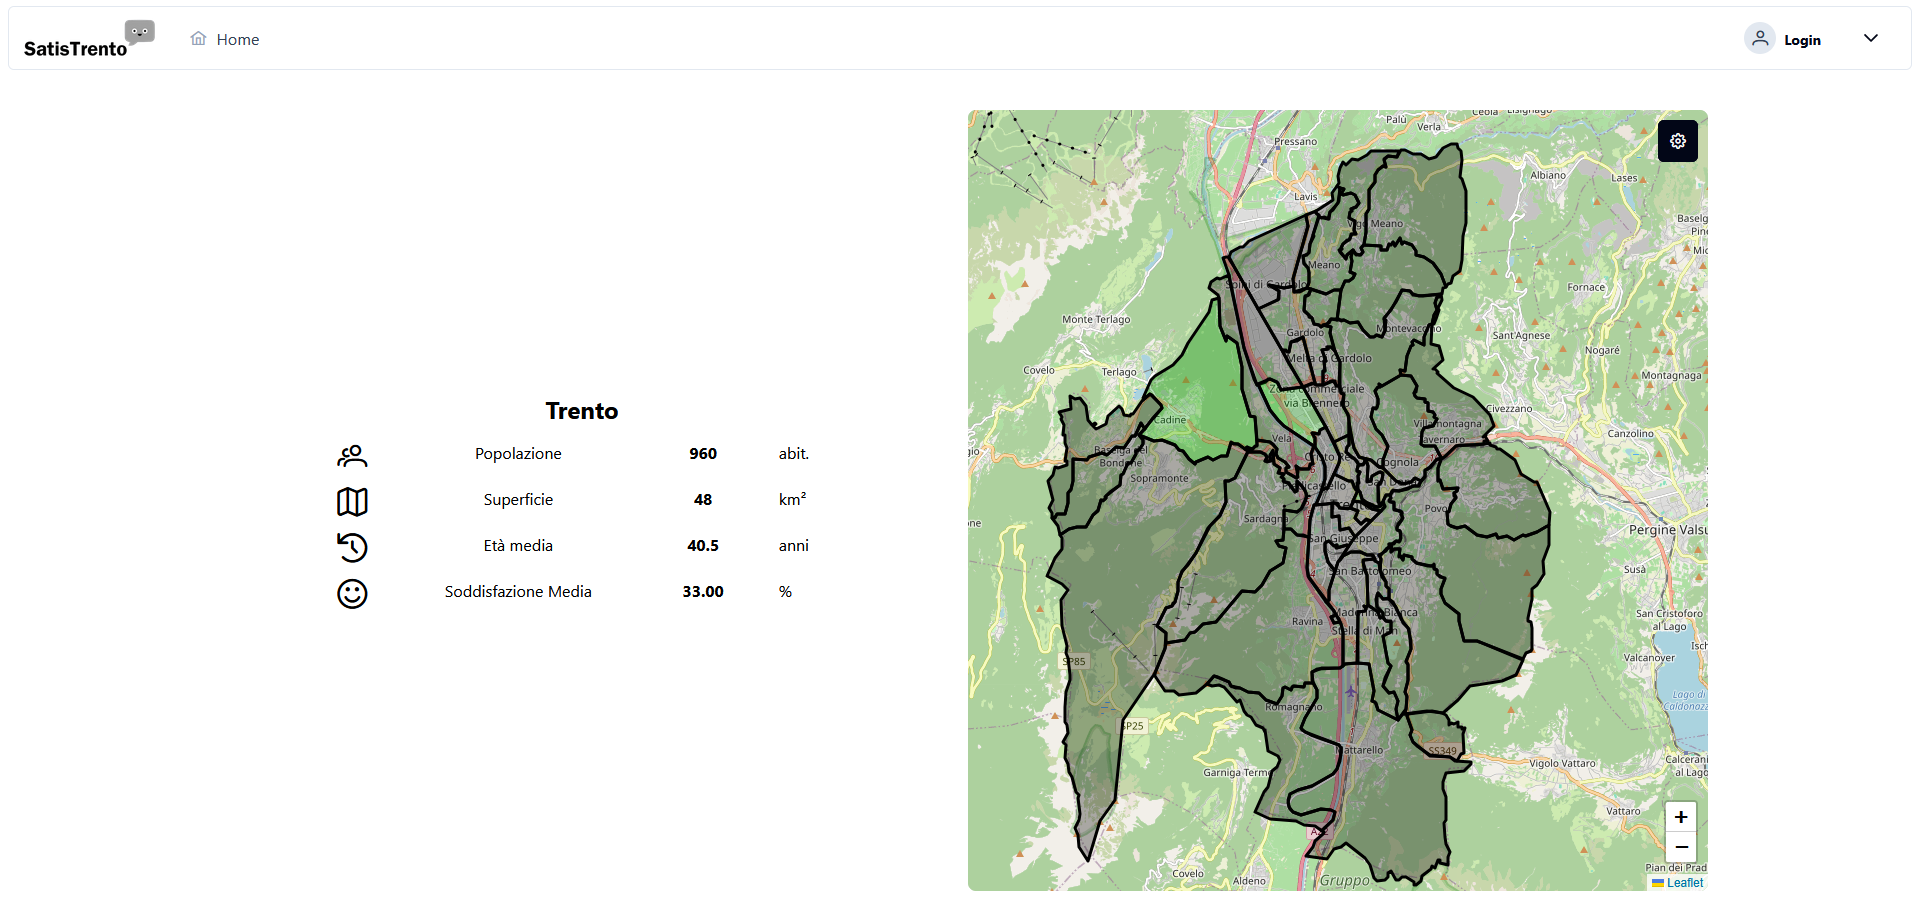
\includegraphics[width=0.8\textwidth]{frontend/home.png}
        \caption{\textit{Home Page} per utenti non loggati}
        \label{fig:frontend-home}
    \end{figure}
    Nella Figura \Ref{fig:frontend-home} è possibile vedere la \textit{Home Page} della \textit{web-app}. Come da specifiche descritte nei documenti precedenti questa presenta: i dati generali relativi all'intero comune, la mappa interattiva, tematica sulla base della soddisfazione media e suddivisa per quartieri. Nell'angolo in alto a destra della mappa è presente un pulsante per aprire il menù delle impostazioni per passare da ``quartieri'' a ``circoscrizioni'' e viceversa. Inoltre, nell'angolo superiore destro della pagina è presente un pulsante per accedere alla pagina di \textit{login}.
    
    \subsubsection{Dettaglio menù impostazioni}
        \begin{figure}[H]
            \centering
            
\includegraphics[width=0.3\textwidth]{frontend/opzioni_quart_circ.png}
            \caption{Menù impostazioni}
            \label{fig:frontend-settings}
        \end{figure}
        Come precedentemente descritto, il menù delle impostazioni sopra raffigurato, chiudibile premendo la ``X'', permette di passare da una visualizzazione dei dati per quartieri ad una per circoscrizioni e viceversa. La figura sopra è relativa a tutte le tipologie di utenti ad eccezione degli utenti con ruolo ``analista''.
\newpage
    \subsubsection{Selezione di un ``quartiere''/``circoscrizione''}
        \begin{figure}[H]
            \centering
            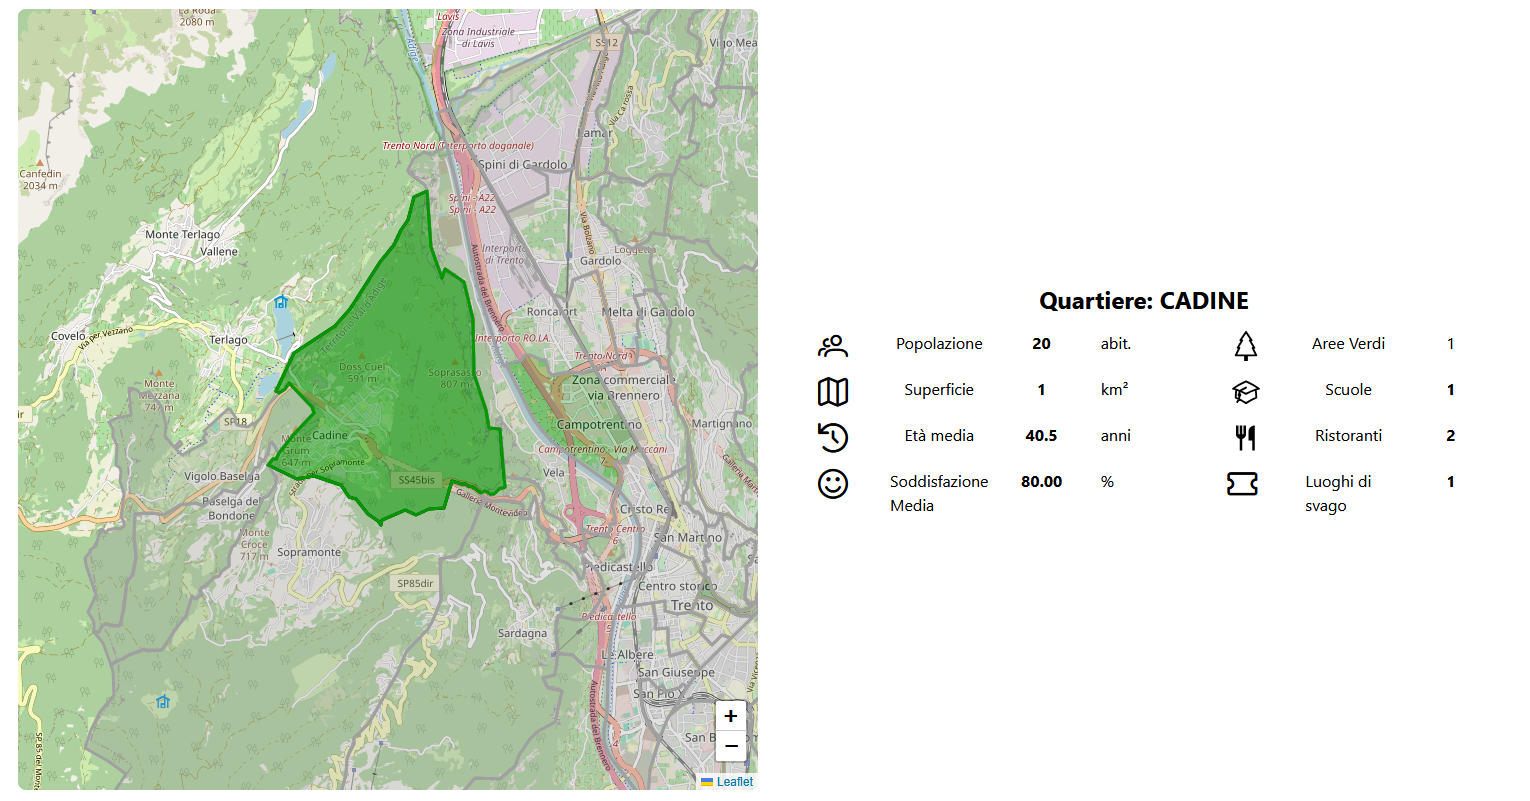
\includegraphics[width=0.8\textwidth]{frontend/quartiere_selezionato.png}
            \caption{Selezione di un ``quartiere''/``circoscrizione''}
            \label{fig:frontend-quartiere}
        \end{figure}
        Notiamo dalla Figura \Ref{fig:frontend-quartiere} come la selezione di un ``quartiere'' o ``circoscrizione'' avvenga tramite un click sulla mappa. Una volta selezionato un ``quartiere'' o ``circoscrizione'' verranno visualizzati degli ulteriori informazioni più specifiche riguardanti il ``quartiere'' o la ``circoscrizione'' selezionata. Inoltre il ``quartiere'' o la ``circoscrizione'' selezionata verrà evidenziata sulla mappa oscurano gli altri ``quartieri'' o le altre ``circoscrizioni'', inoltre la mappa avrà il suo centro sul centro del quartiere ed avrà uno zoom adeguato per visualizzare il ``quartiere'' o la ``circoscrizione'' selezionata nella sua interezza. Da questa schermata è possibile tornare alla visualizzazione generale ri-selezionando il ``quartiere'' o la ``circoscrizione'' selezionata oppure è possibile cambiare ``quartiere'' o ``circoscrizione'' selezionando un altro ``quartiere'' o ``circoscrizione'' dalla mappa.
\section{\textit{Login}}
    \begin{figure}[H]
        \centering
        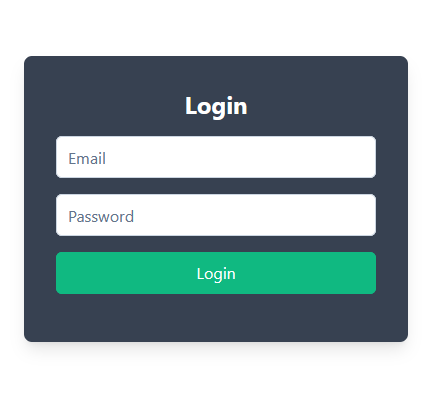
\includegraphics[width=0.4\textwidth]{frontend/dettaglio_login.png}
        \caption{Dettaglio pagina di \textit{login}}
        \label{fig:frontend-login}
    \end{figure}
    Nella Figura \Ref{fig:frontend-login} è possibile vedere il dettaglio della pagina di \textit{login}. Da questa pagina tutti gli utenti in possesso di credenziali valide possono accedere. \newpage
        \subsubsection{Messaggio di errore}
        \begin{figure}[H]
            \centering
            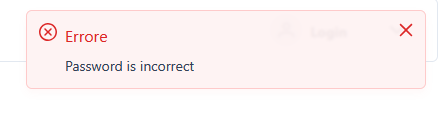
\includegraphics[width=0.4\textwidth]{frontend/dettaglio_errore_login.png}
            \caption{Messaggio di errore}
            \label{fig:frontend-login-error}
        \end{figure}
        Nella Figura \Ref{fig:frontend-login-error} è possibile vedere come si presenta il messaggio di errore in caso di credenziali errate. Questo viene visualizzato per $5$ secondi in caso di credenziali errate o altro errore.\newline
        Si noti come il presente ``formato'' di \textit{feedback} per i messaggi di errori sia stato implementato per tutte le pagine della \textit{web-app} in caso di un qualsiasi errore, viene difatti mostrato il titolo dell'errore con l'azione che non è stata possibile effettuare ed una descrizione più dettagliata del perché non è stato possibile effettuare l'azione richiesta.
        \subsubsection{Messaggio di login effettuato}
        \begin{figure}[H]
            \centering
            
\includegraphics[width=0.4\textwidth]{frontend/dettaglio_messaggio_login.png}
            \caption{Messaggio di login effettuato}
            \label{fig:frontend-login-success}
        \end{figure}
        Nella Figura \Ref{fig:frontend-login-success} è possibile vedere come si presenta il messaggio di login effettuato con successo. Questo viene visualizzato per $3$ secondi in caso di login effettuato con successo.\newline
        Si noti come il presente ``formato'' di \textit{feedback} sia stato implementato per tutte le pagine della \textit{web-app} in caso di un qualsiasi errore, viene difatti mostrato la scritta ``successo'', o altra equivalente, ed una breve descrizione di cosa è stato effettuato con successo.
\section{funzionalità Analista}
    Nella seguente sezione verranno illustrate le funzionalità disponibili per gli utenti con ruolo ``analista''. Questi utenti hanno accesso a funzionalità specifiche per la loro mansione e non disponibili agli altri utenti.
    \begin{figure}[H]
        \centering
        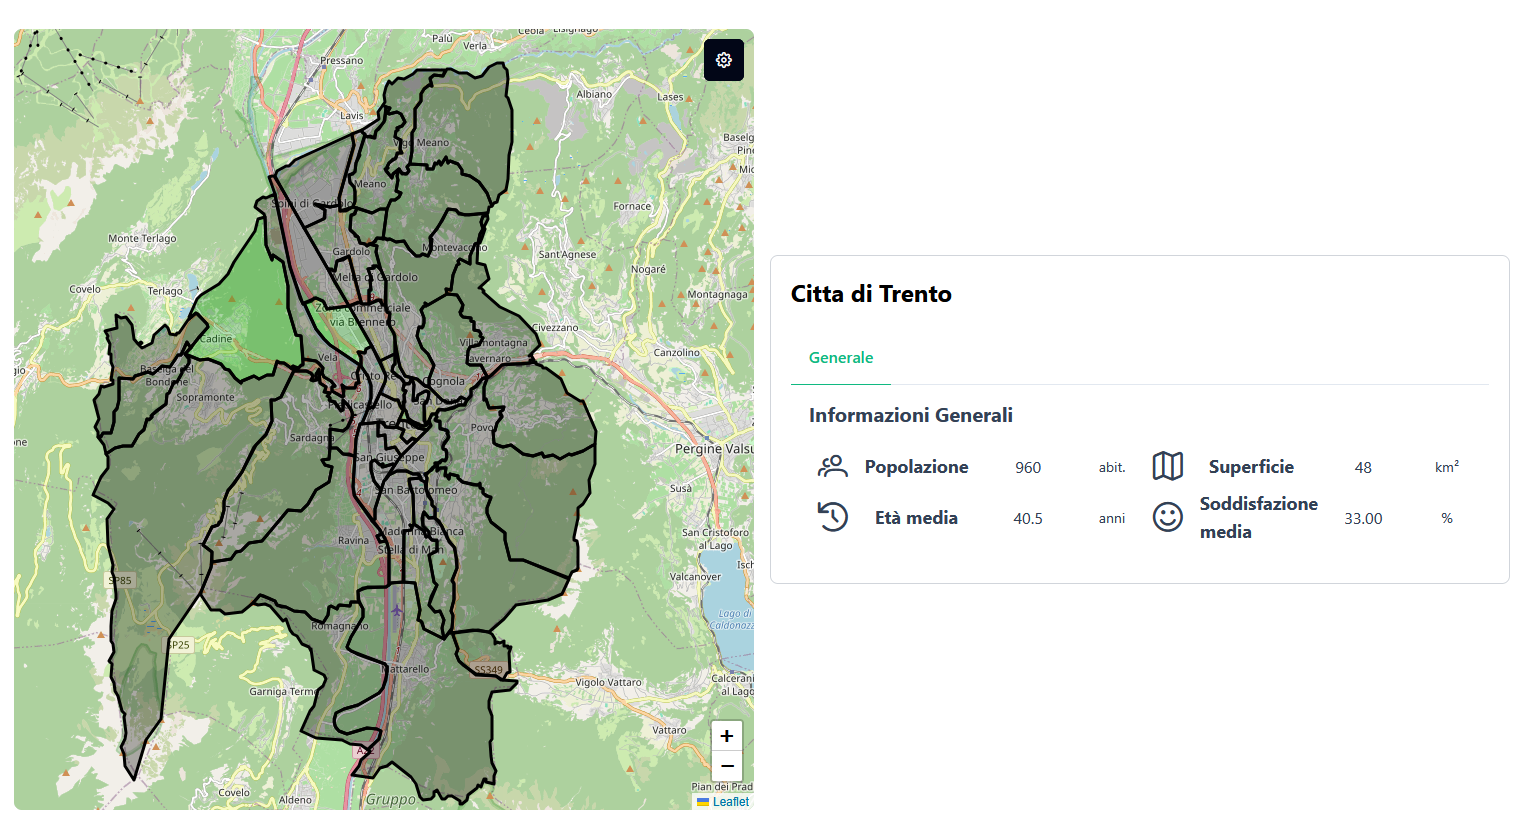
\includegraphics[width=0.8\textwidth]{frontend/home_analista.png}
        \caption{\textit{Home Page} per utenti con ruolo ``analista''}
        \label{fig:frontend-analista}
    \end{figure}
    Possiamo notare dalla Figura \Ref{fig:frontend-analista} come l'interfaccia grafica si sia differenziata rispetto alla Figura \Ref{fig:frontend-home}. Possiamo notare come le informazioni generali del comune siano comunque visibili ma sono raggruppate, non cambia molto infatti dalla \textit{homepage} delle altre tipologie di utenti. 
    \subsubsection{Selezione di un ``quartiere''/``circoscrizione'' - analista}
        \begin{figure}[H]
            \centering
            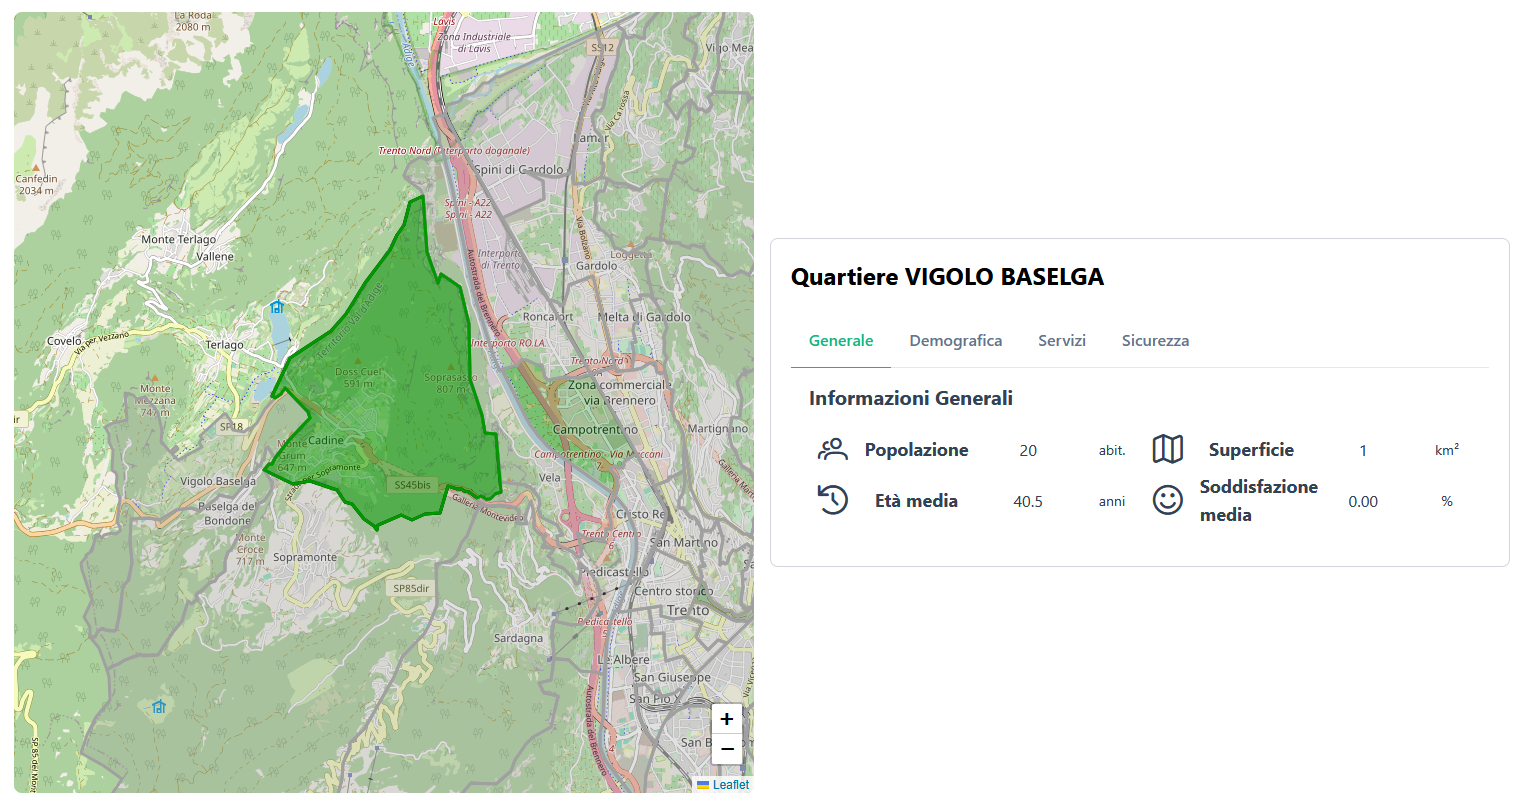
\includegraphics[width=0.8\textwidth]{frontend/alaisi_selezionato.png}
            \caption{Selezione di un ``quartiere''/``circoscrizione'' per utenti con ruolo ``analista''}
            \label{fig:frontend-analista-quartiere}
        \end{figure}
        Notiamo dalla Figura \Ref{fig:frontend-analista-quartiere} come la selezione di un ``quartiere'' o ``circoscrizione'' avvenga tramite un click sulla mappa come nel caso degli altri utenti. Una volta selezionato un ``quartiere'' o ``circoscrizione'' verranno visualizzati oltre alle informazioni generali del ``quartiere'' o della ``circoscrizione'' anche altri indicatori accessibili tramite le diverse pagine del menù posizionato sulla destra della mappa.\newline
        Si possa notare come questa visualizzazione sia una estensione della visualizzazione per gli altri utenti, dunque tutte le funzionalità e le azioni che il sistema compie alla selezione/deselezione sono le stesse.
    \subsubsection{Dettaglio menù impostazioni}
        \begin{figure}[H]
            \centering
            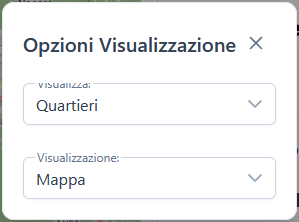
\includegraphics[width=0.3\textwidth]{frontend/opzioni_analista.png}
            \caption{Menù impostazioni per utenti con ruolo ``analista''}
            \label{fig:frontend-settings-analista}
        \end{figure}
        Il menù delle impostazioni per gli utenti con ruolo ``analista'' estende le funzionalità del menù per tutti gli altri utenti della figura \Ref{fig:frontend-settings}. In particolare, oltre alla possibilità di passare da una visualizzazione dei dati per quartieri ad una per circoscrizioni e viceversa, è possibile passare dalla visualizzazione di questi da una visualizzazione in ``mappa'' ad una in ``tabella''. Questo permette agli utenti con ruolo ``analista'' di avere una visione più dettagliata dei dati.
    \subsubsection{Visualizzazione dati in ``tabella''}
        \begin{figure}[H]
            \centering
            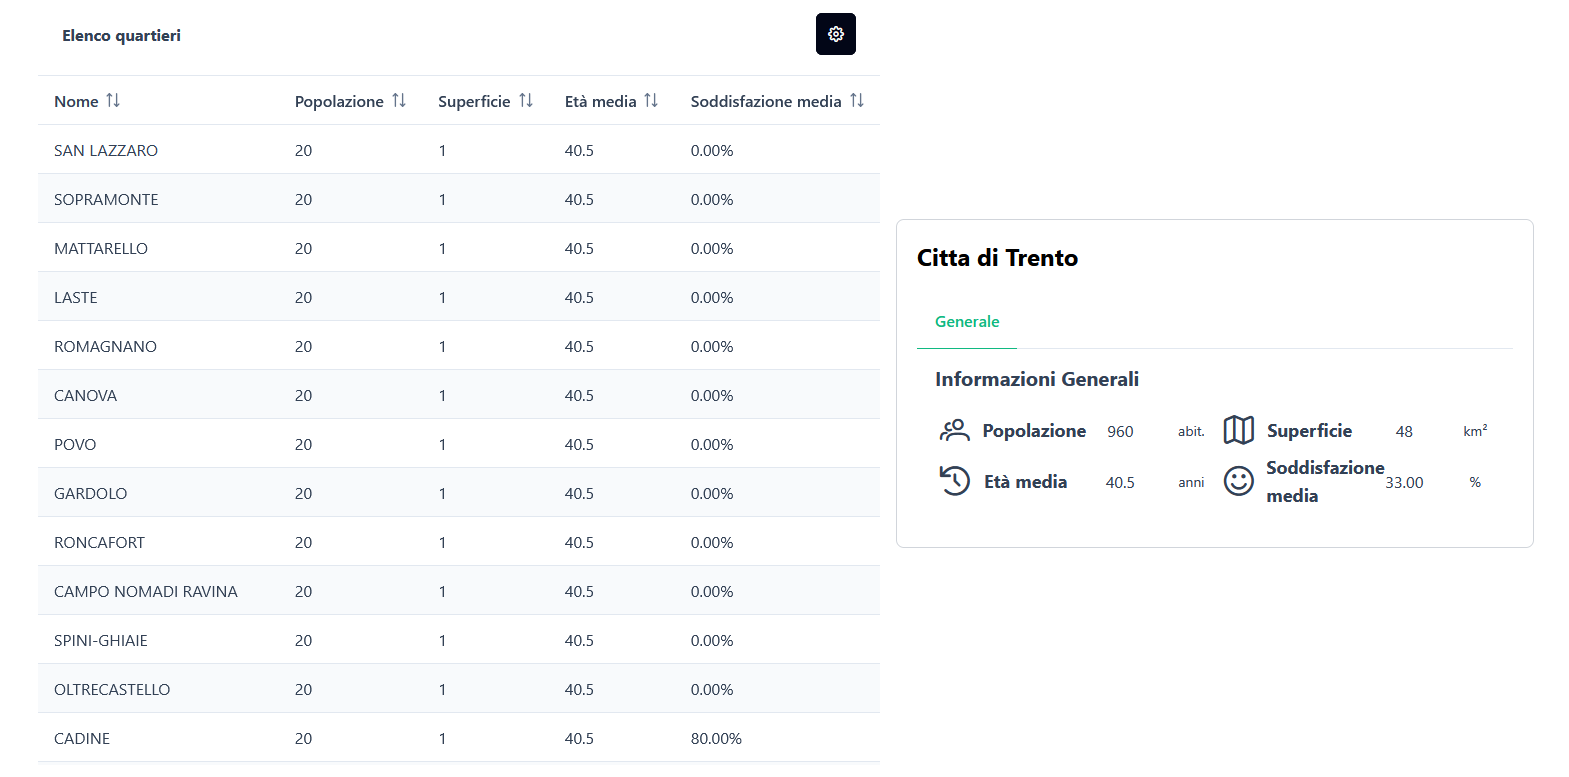
\includegraphics[width=0.8\textwidth]{frontend/home_analista_tabella.png}
            \caption{Visualizzazione dati in ``tabella''}
            \label{fig:frontend-analista-tabella}
        \end{figure}
        Nella Figura \Ref{fig:frontend-analista-tabella} è possibile vedere la visualizzazione dei dati in ``tabella'' per gli utenti con ruolo ``analista''. Questa visualizzazione permette di avere una visione, ordinabile per le colonne presenti, dei dati relativi ai ``quartieri'' o alle ``circoscrizioni''. Da questa visualizzazione è possibile selezionare un ``quartiere'' o una ``circoscrizione'' premendo sulla riga corrispondente. 
    \subsubsection{``Quartiere''/``circoscrizione'' selezionata in visualizzazione tabella}
        \begin{figure}[H]
            \centering
            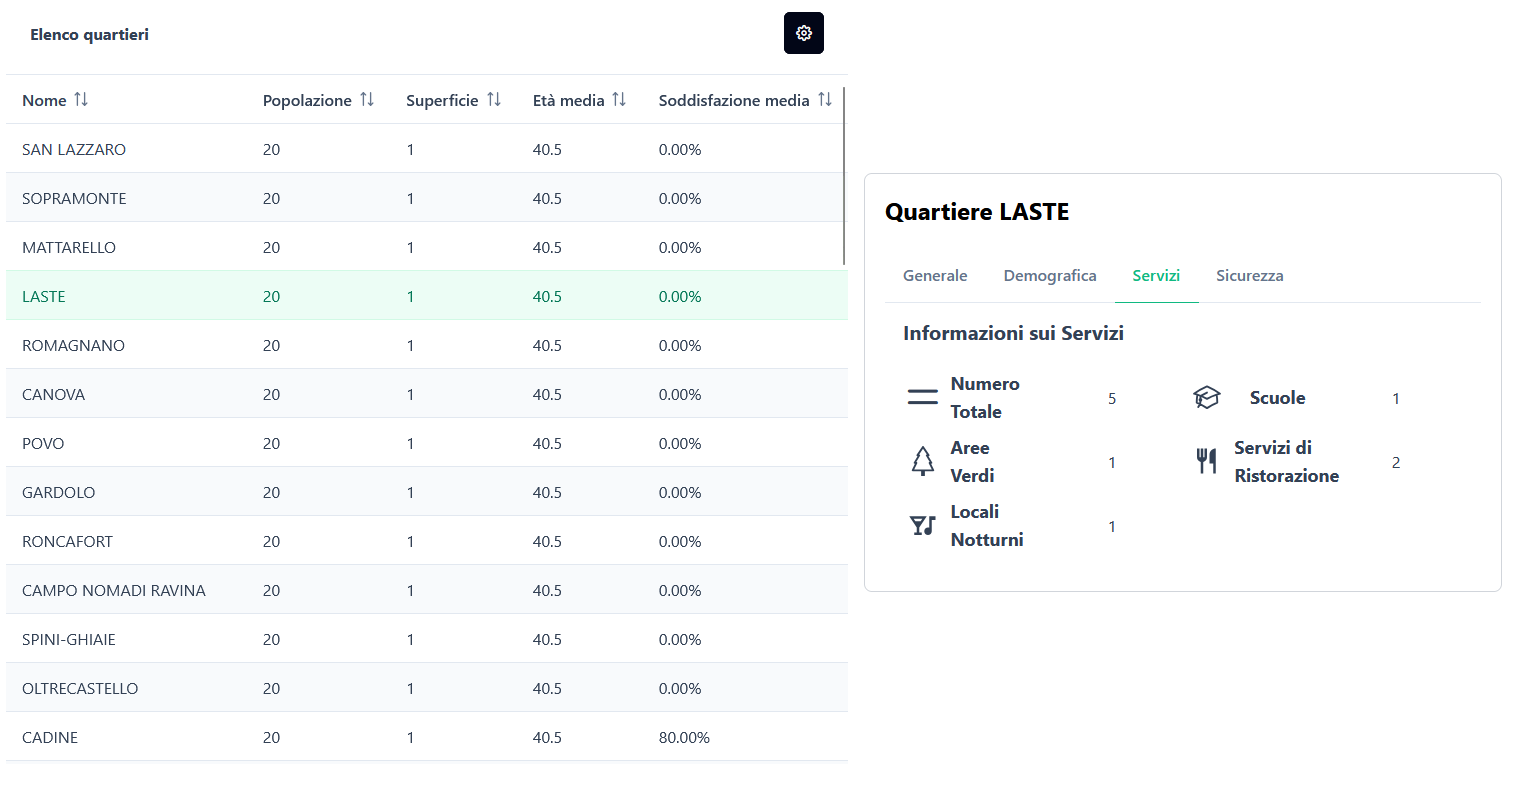
\includegraphics[width=0.8\textwidth]{frontend/alaisi_selezionato_tabella.png}
            \caption{``Quartiere''/``circoscrizione'' selezionata in visualizzazione tabella}
            \label{fig:frontend-analista-tabella-selezionato}
        \end{figure}
        La figura \Ref{fig:frontend-analista-tabella-selezionato} mostra come si presenta la visualizzazione di un ``quartiere'' o una ``circoscrizione'' selezionata in visualizzazione tabella. Questa situazione è una unione della selezione nel caso della figura \Ref{fig:frontend-analista-quartiere} e della visualizzazione in tabella della figura \Ref{fig:frontend-analista-tabella}. Da questa visualizzazione è possibile tornare alla visualizzazione dei dati della città selezionando il ``quartiere'' o la ``circoscrizione'' selezionata oppure è possibile cambiare ``quartiere'' o ``circoscrizione'' selezionando un altro ``quartiere'' o ``circoscrizione'' dalla tabella, in questo caso la riga selezionata verrà evidenziata ed i dati relativi al ``quartiere'' o alla ``circoscrizione'' selezionata verranno visualizzati.
\section{funzionalità Sondaggista}
    \chapter{\textit{Deployment}}

\paragraph{\textit{Live-Demo}} I \textit{deployment} sono stati effettuati su un unico \textit{cluster} di \texttt{render.com} tramite il quale si gestisce anche l'automazione di \texttt{CD}. L'url per accedere all'applicazione è \url{https://satistrento.onrender.com/}. Per accedere alle aree riservate è necessario utilizzare delle credenziali:
\begin{description}
    \item[Utente Sondaggista] \texttt{sondaggista@test.com} - \texttt{password}
    \item[Utente Analista] \texttt{analista@test.com} - \texttt{password}
\end{description}
Altre tipologie di utenti precedentemente definite dai requisiti funzionali non sono state implementate.


\paragraph{\texttt{CI}/\texttt{CD}}
    Come precedentemente descritto il \textit{deployment} è stato automatizzato tramite \texttt{GitHub Actions} e \texttt{render.com}, questo ad ogni commit sul branch \texttt{main} effettua il \textit{deployment} in modo automatico della nuova versione dell'applicazione. \newline
    Per la parte di \texttt{CI} sono stati implementati dei \textit{tests} tramite \texttt{Jest} e \texttt{supertest} per verificare il corretto funzionamento delle \textit{API} e delle funzionalità dell'applicazione, queste sono state automatizzate dal file \texttt{.github/workflows/jestTesting.yml} presente nella repository del progetto, inoltre in quanto si è usato \texttt{TypeScript} è stato scelto di verificare anche la correttezza del codice tramite la \texttt{GitHub Action} definita nel file \texttt{.github/workflows/buildTS.yaml}.

\paragraph{\textit{Help}}
    Per problemi sulla \textit{live-demo} contattare Luca Facchini all'indirizzo \href{mailto:luca.facchini-1@studenti.unitn.it}{luca.facchini-1@studenti.unitn.it} in quanto è il solo abilitato ad accedere alla dashboard di \texttt{render.com} e quindi a poter risolvere eventuali problemi.

    \afterpage{\blankpage}
\end{document}
